% =====================================================================
%  Proyecto Integrador de Métodos Numéricos con MATLAB
%  Analizador numérico de vibraciones con el acelerómetro de un teléfono
%  Formato: APA 7 (modo estudiante) — compilar con LuaLaTeX + Biber:
%      latexmk -lualatex main.tex
%  La portada se entrega por separado (firmada).
% =====================================================================
\documentclass[stu,12pt,a4paper,floatsintext,donotrepeattitle]{apa7}

% ---------- Idioma y tipografía ----------
\usepackage[spanish,es-tabla,es-noshorthands]{babel}
\usepackage{fontspec}
\setmainfont{TeX Gyre Termes}          % equivalente libre de Times New Roman (APA 7: 12 pt)
\setmonofont{DejaVu Sans Mono}[Scale=0.85]
\usepackage{csquotes}
\usepackage[style=apa,backend=biber]{biblatex}
\addbibresource{referencias.bib}

% ---------- Matemáticas, tablas y figuras ----------
\usepackage{amsmath,amssymb}
\usepackage{booktabs,longtable,array,tabularx,multirow}
\usepackage{graphicx}
\graphicspath{{../App/figuras/claro/}{capturas/}}
\usepackage{tikz}
\usetikzlibrary{positioning,arrows.meta,shapes.geometric,fit,calc,backgrounds}
\usepackage{xcolor}
\usepackage{listings}
\usepackage{caption}
\usepackage{hyperref}
\hypersetup{colorlinks=true,linkcolor=black,citecolor=black,urlcolor=blue!50!black}

% ---------- Código MATLAB ----------
\lstdefinestyle{matlab}{
  language=Matlab, basicstyle=\ttfamily\footnotesize, breaklines=true,
  keywordstyle=\color{blue!60!black}\bfseries, commentstyle=\color{green!40!black},
  stringstyle=\color{red!55!black}, numbers=left, numberstyle=\tiny\color{gray},
  frame=single, rulecolor=\color{gray!50}, columns=fullflexible, keepspaces=true,
  showstringspaces=false, extendedchars=true, tabsize=4, xleftmargin=1.5em
}
\lstset{style=matlab}
% Emojis de los botones de la interfaz (sin glifo en la fuente monoespaciada)
\usepackage{newunicodechar}
\newunicodechar{📂}{[carpeta]}\newunicodechar{🧪}{[prueba]}\newunicodechar{💾}{[guardar]}\newunicodechar{📊}{[gráfica]}\newunicodechar{⏸}{[pausa]}

% ---------- Utilidades ----------
\newcommand{\matlab}{MATLAB}
\newcommand{\dd}{\,\mathrm{d}}
% Captura o fotografía: si el archivo existe se inserta; si no, se deja un recuadro
\newcommand{\captura}[3]{%
  \IfFileExists{capturas/#1}{\includegraphics[width=#2]{capturas/#1}}{%
    \fbox{\parbox[c][5.5cm][c]{#2}{\centering\small\textbf{PENDIENTE:} #3\\[4pt]
      \footnotesize Guardar como \texttt{Documento/capturas/\detokenize{#1}}}}}}

\title{Analizador numérico de vibraciones con el acelerómetro de un teléfono}
\shorttitle{}  % APA 7 estudiante: sin encabezado, solo número de página
\author{José Ricardo Pacheco}
\affiliation{Universidad Anáhuac Mayab}
\course{Métodos Numéricos}
\professor{}
\duedate{Diciembre de 2026}

\begin{document}

% La portada firmada se entrega por separado (instrucciones del proyecto).
\section*{Resumen}
\addcontentsline{toc}{section}{Resumen}

Se desarrolló en \matlab{} una aplicación con interfaz gráfica para analizar numéricamente señales de aceleración medidas con el acelerómetro de un teléfono inteligente. El caso de estudio fue la vibración de un automóvil Kia Forte L 2019 con motor de cuatro cilindros. Se midió con un iPhone 15 Pro Max y la aplicación phyphox a 100~Hz, en tres condiciones: sobre el cofre con el motor en ralentí, sobre el descansabrazos de la cabina con el vehículo estacionado y sobre el tablero durante la conducción.

La aplicación calcula la duración de la señal, detecta datos faltantes y valores atípicos (filtro de Hampel) y reconstruye la señal sobre una malla uniforme por interpolación lineal, polinomial de Newton o trazador cúbico natural. Además obtiene la derivada con cuatro esquemas de diferencias finitas, integra con las reglas del trapecio y de Simpson 1/3 y 3/8, resuelve la ecuación diferencial del movimiento con Euler, Heun y Runge-Kutta de cuarto orden, y ajusta líneas de tendencia por mínimos cuadrados que también sirven para corregir la deriva del sensor. Incluye reproducción en tiempo real con grabación controlada por el usuario y exportación de resultados con nombre de archivo elegido.

Todos los métodos se validaron contra una señal con solución analítica: los órdenes de convergencia observados (1.00, 2.00 y 3.99 para las derivadas; 2.00 y 4.00 para las integrales; 1.11, 2.00 y 3.94 para la ecuación diferencial) coinciden con la teoría. Con datos reales, la frecuencia dominante de 25.26~Hz corresponde a unas 758~rpm de ralentí con el motor frío y bajó a 22.86~Hz (686~rpm) al calentarse. Este valor coincide con el de phyphox con una diferencia de 0.2~Hz.

La corrección de deriva por mínimos cuadrados redujo el desplazamiento falso del vehículo estacionado de 127~m a 0.31~m. Con la vibración real la interpolación lineal superó al trazador cúbico, porque la señal tiene cerca de cuatro muestras por ciclo; en una señal suave ocurre lo contrario. Por eso se concluye que el método más efectivo depende de la relación entre la frecuencia de la señal y la de muestreo.

\textit{Palabras clave:} métodos numéricos, interpolación, diferenciación numérica, integración numérica, Runge-Kutta, mínimos cuadrados, acelerómetro, vibraciones, \matlab{}.

\clearpage

\tableofcontents
\clearpage
\section{Introducción}

Los teléfonos inteligentes traen sensores de movimiento (acelerómetro, giroscopio y magnetómetro) que, con una aplicación adecuada, funcionan como instrumentos de medición de bajo costo. La aplicación phyphox fue diseñada para usar esos sensores en experimentos de física y permite exportar los datos crudos para analizarlos fuera del teléfono \parencite{staacks2018}. Una señal de aceleración real, sin embargo, no puede usarse tal cual. El muestreo es discreto y puede perder muestras, el sensor tiene un sesgo que se acumula al integrar, aparecen picos espurios y la información útil (la velocidad, el desplazamiento o la frecuencia de vibración) solo se obtiene después de derivar, integrar o ajustar los datos. Estas tareas son justamente el campo de los métodos numéricos \parencite{chapra2015}.

Este proyecto integra en una sola herramienta los algoritmos del curso para resolver un problema real de ingeniería: caracterizar la vibración de un automóvil a partir de mediciones con un teléfono. El sistema físico elegido, autorizado por el profesor, es un Kia Forte L 2019 con motor de cuatro cilindros. Un motor de combustión de cuatro tiempos produce una vibración periódica cuya frecuencia depende de su velocidad de giro, así que medir esa frecuencia permite estimar las revoluciones por minuto sin un tacómetro.

\subsection{Planteamiento del problema}

Se requiere una interfaz gráfica en \matlab{} que, a partir de un archivo de datos de aceleración, realice los procesos solicitados: duración total de la señal, detección e interpolación de datos faltantes, derivada, integral y línea de tendencia por mínimos cuadrados. Debe permitir elegir algoritmos y parámetros, graficar los datos originales y procesados, mostrar los valores obtenidos y guardar los resultados en un archivo cuyo nombre indique el usuario, quien además controla el inicio y el fin de la grabación de la señal en tiempo real.

\subsection{Objetivos}

\subsubsection{Objetivo general}
Desarrollar una aplicación en \matlab{} que integre interpolación, diferenciación, integración, solución de ecuaciones diferenciales y mínimos cuadrados para analizar la vibración real de un automóvil medida con un teléfono, y justificar con evidencia cuantitativa qué métodos resultan más efectivos.

\subsubsection{Objetivos específicos}
\begin{enumerate}
  \item Implementar los métodos numéricos sin depender de las funciones equivalentes de \matlab{} y validarlos contra una solución analítica, comprobando su orden de convergencia.
  \item Detectar y reconstruir datos faltantes y valores atípicos en señales medidas.
  \item Estimar la frecuencia de vibración del motor y relacionarla con su velocidad de giro.
  \item Obtener velocidad y desplazamiento por integración y corregir la deriva del sensor con mínimos cuadrados.
  \item Construir una interfaz con carga de datos, menús de algoritmos, gráficas, indicadores, reproducción en tiempo real y exportación de resultados.
\end{enumerate}

\subsection{Alcance}
Se analizan tres mediciones reales de alrededor de un minuto cada una, tomadas con el mismo teléfono a una frecuencia de muestreo de 100~Hz, y una señal sintética con solución conocida. La herramienta acepta archivos CSV y Excel exportados por phyphox, archivos MAT de \matlab{} Mobile y tablas genéricas cuya primera columna sea el tiempo. Queda fuera del alcance la fusión de sensores (acelerómetro con giroscopio) para corregir la orientación del teléfono durante la conducción.

\section{Marco teórico}

\subsection{Señales muestreadas}

Una señal medida es un conjunto de pares $(t_k, y_k)$, $k = 0,1,\dots,N$. Cuando el paso de muestreo $h$ es constante, $t_k = t_0 + kh$ y la frecuencia de muestreo es $f_s = 1/h$. La duración total de la señal es
\begin{equation}
  T = t_N - t_0 .
  \label{eq:duracion}
\end{equation}
Como los tiempos reales presentan pequeñas variaciones (\textit{jitter}), en este trabajo el paso nominal se estima con la mediana de las diferencias, $h = \operatorname{mediana}(t_{k+1} - t_k)$, que no se ve afectada por huecos aislados.

El teorema de muestreo establece que una señal de banda limitada queda determinada por sus muestras solo si su frecuencia máxima cumple $f_{\max} < f_s/2$ \parencite{shannon1949}. A $f_s/2$ se le llama frecuencia de Nyquist. Con $f_s = 100$~Hz, cualquier vibración por encima de 50~Hz aparece en una frecuencia falsa (\textit{aliasing}). Una relación útil para todo el análisis es el número de muestras por ciclo, $f_s/f$. Para la vibración del motor ($f \approx 25$~Hz) es de apenas cuatro, un dato que explica varios de los resultados de la sección~\ref{sec:analisis}.

\subsection{Detección de datos faltantes y valores atípicos}

Se distinguen tres tipos de dato faltante:
\begin{enumerate}
  \item \textit{Valores no numéricos} (NaN), es decir, muestras perdidas o corruptas.
  \item \textit{Huecos temporales}: muestras eliminadas, detectadas cuando
  \begin{equation}
    t_{k+1} - t_k > c \cdot h, \qquad c = 1.5 .
  \end{equation}
  \item \textit{Valores atípicos}: muestras físicamente imposibles que conviene tratar como faltantes. Se detectan con el filtro de Hampel, basado en estadísticos robustos \parencite{hampel1974}. Para cada muestra se toma una ventana de $2k+1$ valores y se calculan
  \begin{equation}
    m_i = \operatorname{mediana}\{y_{i-k},\dots,y_{i+k}\}, \qquad
    S_i = 1.4826 \cdot \operatorname{mediana}\{|y_j - m_i|\} ,
  \end{equation}
  y la muestra se declara atípica si $|y_i - m_i| > n_\sigma S_i$ (aquí $k = 25$ y $n_\sigma = 5$). El factor 1.4826 hace que $S_i$ estime la desviación estándar de una distribución normal. A diferencia de la desviación estándar, $S_i$ no se contamina con el propio valor atípico.
\end{enumerate}

\subsection{Interpolación}

Los puntos faltantes de una malla uniforme $t_0, t_0 + h, \dots$ se reconstruyen a partir de las muestras válidas $(x_i, y_i)$.

\paragraph{Interpolación lineal.} Para $x_i \le x \le x_{i+1}$,
\begin{equation}
  p(x) = y_i + \frac{y_{i+1} - y_i}{x_{i+1} - x_i}\,(x - x_i).
\end{equation}

\paragraph{Polinomio de Newton en diferencias divididas.} Con $n+1$ nodos,
\begin{equation}
  p_n(x) = f[x_0] + f[x_0,x_1](x - x_0) + \dots + f[x_0,\dots,x_n]\prod_{j=0}^{n-1}(x - x_j),
\end{equation}
donde $f[x_i,\dots,x_{i+m}] = \bigl(f[x_{i+1},\dots,x_{i+m}] - f[x_i,\dots,x_{i+m-1}]\bigr)/(x_{i+m} - x_i)$ \parencite{chapra2015}. Un polinomio global de grado alto oscila entre nodos (fenómeno de Runge), por lo que se usa un polinomio \emph{local} de grado 3, construido con los cuatro nodos más cercanos al punto a interpolar y evaluado con el esquema de Horner.

\paragraph{Trazador cúbico natural.} En cada intervalo $[x_i, x_{i+1}]$, con $h_i = x_{i+1} - x_i$ y $M_i = S''(x_i)$,
\begin{equation}
  S_i(x) = A\,y_i + B\,y_{i+1} + \frac{(A^3 - A)M_i + (B^3 - B)M_{i+1}}{6}\,h_i^2,
  \qquad A = \frac{x_{i+1} - x}{h_i},\; B = 1 - A .
\end{equation}
La continuidad de la primera derivada lleva al sistema tridiagonal
\begin{equation}
  h_{i-1}M_{i-1} + 2(h_{i-1} + h_i)M_i + h_i M_{i+1}
  = 6\left(\frac{y_{i+1} - y_i}{h_i} - \frac{y_i - y_{i-1}}{h_{i-1}}\right),
  \qquad M_0 = M_n = 0 ,
  \label{eq:spline}
\end{equation}
que se resuelve en $O(n)$ operaciones con el algoritmo de Thomas, una eliminación gaussiana especializada para matrices tridiagonales \parencite{burden2017}.

\subsection{Diferenciación numérica}

A partir de la serie de Taylor se obtienen las fórmulas de diferencias finitas \parencite{chapra2015}:
\begin{align}
  \text{Adelante:}\quad & f'(x) \approx \frac{f(x+h) - f(x)}{h}, & E &= O(h), \\
  \text{Atrás:}\quad & f'(x) \approx \frac{f(x) - f(x-h)}{h}, & E &= O(h), \\
  \text{Centrada:}\quad & f'(x) \approx \frac{f(x+h) - f(x-h)}{2h}, & E &= O(h^2), \\
  \text{Cinco puntos:}\quad & f'(x) \approx \frac{-f(x+2h) + 8f(x+h) - 8f(x-h) + f(x-2h)}{12h}, & E &= O(h^4).
\end{align}
En los extremos de la señal se usan fórmulas unilaterales del mismo orden, por ejemplo $f'(x_0) \approx (-3f_0 + 4f_1 - f_2)/(2h)$.

El orden indica cómo disminuye el error al reducir $h$, pero en una señal muestreada $h$ es fijo. Para una oscilación $f(t) = e^{i\omega t}$, cada fórmula devuelve la derivada exacta multiplicada por un factor que depende de $\theta = \omega h$:
\begin{equation}
  |G_{\text{adel}}| = \frac{2\sin(\theta/2)}{\theta}, \qquad
  G_{\text{cent}} = \frac{\sin\theta}{\theta}, \qquad
  G_{5} = \frac{8\sin\theta - \sin 2\theta}{6\theta} .
  \label{eq:factor}
\end{equation}
Un factor menor que 1 significa que la derivada numérica subestima la amplitud real; la fórmula de adelante, además, introduce un desfase de $\theta/2$.

\subsection{Integración numérica}

Con $n$ intervalos de ancho $h$ \parencite{chapra2015}:
\begin{align}
  \text{Trapecio:}\quad & I \approx \frac{h}{2}\Bigl[f_0 + 2\sum_{i=1}^{n-1} f_i + f_n\Bigr], & E &= O(h^2), \\
  \text{Simpson 1/3:}\quad & I \approx \frac{h}{3}\Bigl[f_0 + 4\!\!\sum_{i\ \text{impar}}\!\! f_i + 2\!\!\sum_{i\ \text{par}}\!\! f_i + f_n\Bigr], & E &= O(h^4), \\
  \text{Simpson 3/8:}\quad & I \approx \frac{3h}{8}\bigl[f_0 + 3f_1 + 3f_2 + 2f_3 + \dots + f_n\bigr], & E &= O(h^4).
\end{align}
Simpson 1/3 requiere un número par de intervalos y Simpson 3/8, un múltiplo de tres. Cuando no se cumple esa condición, el residuo se integra con la otra regla de Simpson para conservar el orden $O(h^4)$.

Para la integral acumulada $\int_{t_0}^{t_k} f\dd t$, que es la velocidad cuando $f$ es una aceleración, cada intervalo se integra con la parábola que pasa por tres nodos vecinos:
\begin{equation}
  \int_{x_0}^{x_1} f\dd x \approx \frac{h}{12}\bigl(5f_0 + 8f_1 - f_2\bigr),
  \qquad
  \int_{x_1}^{x_2} f\dd x \approx \frac{h}{12}\bigl(-f_0 + 8f_1 + 5f_2\bigr).
\end{equation}
La suma de ambos tramos es exactamente la regla de Simpson 1/3.

\subsection{Ecuaciones diferenciales ordinarias}

La cinemática del teléfono a partir de la aceleración medida $a(t)$ es el sistema
\begin{equation}
  \frac{\dd x}{\dd t} = v, \qquad \frac{\dd v}{\dd t} = a(t), \qquad x(t_0) = 0,\; v(t_0) = 0 .
  \label{eq:edo}
\end{equation}
Con $\mathbf{y} = (x, v)^T$ y $\mathbf{f}(t,\mathbf{y}) = (v, a(t))^T$ se aplican los métodos \parencite{chapra2015,burden2017}:
\begin{align}
  \text{Euler:}\quad & \mathbf{y}_{k+1} = \mathbf{y}_k + h\,\mathbf{f}(t_k,\mathbf{y}_k), \qquad O(h), \\
  \text{Heun:}\quad & \mathbf{y}_{k+1} = \mathbf{y}_k + \tfrac{h}{2}\bigl[\mathbf{f}(t_k,\mathbf{y}_k) + \mathbf{f}(t_{k+1},\mathbf{y}_k + h\mathbf{f}(t_k,\mathbf{y}_k))\bigr], \qquad O(h^2), \\
  \text{RK4:}\quad & \mathbf{y}_{k+1} = \mathbf{y}_k + \tfrac{h}{6}\bigl(\mathbf{k}_1 + 2\mathbf{k}_2 + 2\mathbf{k}_3 + \mathbf{k}_4\bigr), \qquad O(h^4),
\end{align}
con $\mathbf{k}_1 = \mathbf{f}(t_k,\mathbf{y}_k)$, $\mathbf{k}_2 = \mathbf{f}(t_k + h/2, \mathbf{y}_k + h\mathbf{k}_1/2)$, $\mathbf{k}_3 = \mathbf{f}(t_k + h/2, \mathbf{y}_k + h\mathbf{k}_2/2)$ y $\mathbf{k}_4 = \mathbf{f}(t_k + h, \mathbf{y}_k + h\mathbf{k}_3)$. RK4 necesita $a(t_k + h/2)$, un instante donde no hay muestra; ese valor se obtiene con el polinomio de Newton local de grado 3.

\subsection{Mínimos cuadrados}

La línea de tendencia de grado $g$ minimiza $S_r = \sum_i \bigl(y_i - p(t_i)\bigr)^2$. Para evitar el mal condicionamiento de la matriz de Vandermonde se usa la variable escalada $s = (t - \mu)/\sigma$ y el modelo $p(s) = \sum_{j=0}^{g} a_j s^j$. Los coeficientes resuelven las ecuaciones normales
\begin{equation}
  \bigl(\mathbf{Z}^T\mathbf{Z}\bigr)\,\mathbf{a} = \mathbf{Z}^T\mathbf{y}, \qquad Z_{ij} = s_i^{\,j},
  \label{eq:normales}
\end{equation}
mediante eliminación gaussiana con pivoteo parcial \parencite{chapra2015}. La calidad del ajuste se mide con
\begin{equation}
  R^2 = 1 - \frac{S_r}{S_t}, \qquad S_t = \sum_i (y_i - \bar y)^2, \qquad
  S_{y/x} = \sqrt{\frac{S_r}{n - (g+1)}} .
\end{equation}
El caso $g = 0$ es la media de los datos.

\subsection{Deriva del acelerómetro}
\label{sec:deriva}

Si el sensor mide $a_m(t) = a(t) + b$, con un sesgo constante $b$, al integrar dos veces el error crece como
\begin{equation}
  \Delta v(t) = b\,t, \qquad \Delta x(t) = \tfrac{1}{2}\,b\,t^2 .
  \label{eq:deriva}
\end{equation}
Un sesgo de apenas $0.064$~m/s$^2$ durante 64~s produce $\Delta x \approx 131$~m. Por eso, antes de integrar, se resta un modelo del sesgo obtenido por mínimos cuadrados: de grado 0 (sesgo constante), de grado 1 (sesgo más deriva térmica lineal) o la media de un intervalo inicial en reposo.

\subsection{Análisis espectral y velocidad del motor}

La transformada discreta de Fourier descompone la señal en frecuencias $f_m = m/(Nh)$, con resolución $\Delta f = 1/T$. Se calcula con el algoritmo FFT \parencite{cooley1965}. En un motor de cuatro tiempos cada cilindro produce una explosión cada dos vueltas del cigüeñal, de modo que la frecuencia de encendido y la velocidad de giro se relacionan por
\begin{equation}
  f = \frac{\text{rpm}}{60}\cdot\frac{n_{\text{cil}}}{2}
  \quad\Longrightarrow\quad
  \text{rpm} = \frac{120\,f}{n_{\text{cil}}} ,
  \label{eq:rpm}
\end{equation}
que para el motor de cuatro cilindros del caso de estudio se reduce a $\text{rpm} = 30f$.

\section{Metodología}

\subsection{Sistema físico e instrumentación}

El sistema analizado es un automóvil Kia Forte L 2019 con motor de gasolina de cuatro cilindros. Todo el procesamiento se programó en \matlab{} \parencite{matlab}. Las mediciones se tomaron con un iPhone 15 Pro Max (identificador de modelo iPhone16,2, registrado en los metadatos del archivo) y la aplicación phyphox 1.2.1, usando el experimento \textit{Acceleration (without g)}, que entrega la aceleración lineal sin la componente de gravedad en los tres ejes del teléfono \parencite{staacks2018}. En el iPhone el eje $x$ es lateral, el $y$ va a lo largo de la pantalla y el $z$ es perpendicular a ella. Como verificación independiente se registró también el experimento \textit{Acceleration Spectrum} de la misma aplicación, que calcula su propio espectro de frecuencia.

\begin{table}[htbp]
\caption{Mediciones realizadas el 24 de noviembre de 2026}
\label{tab:mediciones}
\centering\small
\begin{tabular}{@{}lp{6.2cm}cccc@{}}
\toprule
Archivo & Condición & Inicio & $T$ [s] & $N$ & $f_s$ [Hz] \\
\midrule
\texttt{motor\_ralenti\_cofre} & Estacionado, ralentí recién encendido, teléfono sobre el cofre & 11:22 & 63.97 & 6\,397 & 100.0 \\
\texttt{manejo\_tablero} & En circulación, teléfono sobre el tablero & 11:28 & 78.52 & 7\,851 & 100.0 \\
\texttt{motor\_ralenti\_cabina} & Estacionado, ralentí, teléfono sobre la tapa del descansabrazos & 11:53 & 63.54 & 6\,353 & 100.0 \\
\bottomrule
\end{tabular}
\figurenote{Las tres mediciones se exportaron desde phyphox en formato Excel y se convirtieron también a CSV. $T$: duración total; $N$: número de muestras; $f_s$: frecuencia de muestreo nominal.}
\end{table}

\begin{figure}[htbp]
\caption{Montaje del teléfono durante las mediciones}
\label{fig:montaje}
\centering
\captura{montaje_cofre.jpg}{0.45\linewidth}{fotografía del teléfono sobre el cofre}\hfill
\captura{montaje_cabina.jpg}{0.45\linewidth}{fotografía del teléfono sobre el descansabrazos}
\figurenote{Izquierda: medición sobre el cofre. Derecha: medición en la cabina.}
\end{figure}

\subsection{Protocolo de medición}

Las mediciones con el vehículo estacionado se hicieron con el teléfono fijo, boca arriba y lejos de fuentes de calor. Primero se tomó la del cofre, con el motor recién encendido, y unos 30 minutos después la de la cabina, ya con el motor caliente. La medición en circulación se hizo con el teléfono sobre el tablero, sin que el conductor lo manipulara. El protocolo completo, con las recomendaciones de seguridad, está en el archivo \texttt{protocolo\_medicion.md} del repositorio.

\subsection{Arquitectura del programa}

El programa separa la interfaz de la matemática en tres capas:
\begin{enumerate}
  \item \textbf{Interfaz} (\texttt{AnalizadorVibracionesApp.m}): una clase que hereda de \texttt{matlab.apps.AppBase}, la misma estructura que genera App Designer \parencite{mathworks_onramp}. Contiene los componentes, sus funciones de respuesta, la reproducción en tiempo real y la exportación.
  \item \textbf{Motor} (\texttt{nm\_procesar.m}): ejecuta la cadena completa de cálculo y devuelve una estructura con todos los resultados. Como no depende de la interfaz, puede probarse automáticamente.
  \item \textbf{Métodos} (\texttt{metodos/nm\_*.m}): una función por algoritmo, programada sin recurrir a \texttt{interp1}, \texttt{gradient}, \texttt{trapz}, \texttt{ode45} ni \texttt{polyfit}. Esas funciones de \matlab{} se usan solo para comparar resultados.
\end{enumerate}

\begin{table}[htbp]
\caption{Funciones numéricas implementadas}
\label{tab:funciones}
\centering\small
\begin{tabular}{@{}lp{9.4cm}@{}}
\toprule
Función & Método / propósito \\
\midrule
\texttt{nm\_duracion} & Duración total, número de muestras, paso y frecuencia de muestreo (ec.~\ref{eq:duracion}) \\
\texttt{nm\_detectar\_faltantes} & NaN, huecos temporales y atípicos; malla uniforme de reconstrucción \\
\texttt{nm\_hampel} & Filtro de Hampel local (mediana y MAD en ventana móvil) \\
\texttt{nm\_interpolar}, \texttt{nm\_evaluar\_interp} & Reconstrucción por interpolación lineal, Newton local o trazador natural \\
\texttt{nm\_lagrange\_local} & Polinomio de Newton en diferencias divididas con esquema de Horner \\
\texttt{nm\_spline\_natural}, \texttt{nm\_thomas} & Trazador cúbico natural; sistema tridiagonal (ec.~\ref{eq:spline}) \\
\texttt{nm\_derivada} & Diferencias hacia adelante, atrás, centradas y de cinco puntos \\
\texttt{nm\_integral} & Trapecio, Simpson 1/3 y 3/8 compuestos; integral acumulada \\
\texttt{nm\_edo\_movimiento} & Euler, Heun y RK4 para el sistema (ec.~\ref{eq:edo}) \\
\texttt{nm\_minimos\_cuadrados}, \texttt{nm\_gauss\_pivoteo} & Ecuaciones normales con variable escalada; eliminación gaussiana con pivoteo \\
\texttt{nm\_simular\_perdida} & Elimina muestras reales en ráfagas para medir el error de interpolación \\
\texttt{nm\_senal\_prueba} & Señal sintética con solución analítica \\
\texttt{nm\_comparar\_metodos} & Ejecuta todos los métodos y los compara contra la solución analítica y contra \matlab{} \\
\texttt{nm\_cargar\_datos} & Lectura de CSV/XLSX de phyphox, MAT de \matlab{} Mobile y tablas genéricas \\
\bottomrule
\end{tabular}
\end{table}

\subsection{Diagrama de bloques}

La Figura~\ref{fig:bloques} muestra el flujo de datos. La señal cargada pasa por la detección de faltantes y atípicos y se reconstruye sobre una malla uniforme, requisito de las fórmulas de diferencias finitas y de las reglas de Simpson. Sobre esa señal uniforme se calculan, en paralelo, la derivada, la tendencia por mínimos cuadrados y el espectro. La tendencia se resta antes de integrar y de resolver la ecuación diferencial. Todos los resultados alimentan las gráficas, los indicadores, el monitor en tiempo real y la exportación.

\begin{figure}[htbp]
\caption{Diagrama de bloques del analizador}
\label{fig:bloques}
\centering
\begingroup\linespread{1}\selectfont\hyphenpenalty=10000
\begin{tikzpicture}[
  node distance=6mm and 8mm,
  blq/.style={draw, rounded corners=2pt, align=center, font=\footnotesize\linespread{1}\selectfont, minimum height=10mm, text width=30mm, inner sep=3pt, fill=blue!6},
  ent/.style={blq, fill=gray!12},
  sal/.style={blq, fill=green!8},
  dec/.style={blq, fill=orange!10},
  flecha/.style={-{Stealth[length=2mm]}, thick}
]
\node[ent] (arch) {Archivo de datos\\ \scriptsize CSV / XLSX / MAT};
\node[blq, right=of arch] (carga) {Carga y selección de eje\\ \scriptsize \texttt{nm\_cargar\_datos}};
\node[blq, right=of carga] (dur) {Duración y muestreo\\ \scriptsize $T$, $N$, $h$, $f_s$};
\node[blq, below=of dur] (falt) {Detección de faltantes\\ \scriptsize NaN, huecos, Hampel};
\node[dec, left=of falt] (interp) {Interpolación\\ \scriptsize lineal / Newton / spline};
\node[blq, left=of interp] (malla) {Señal uniforme\\ \scriptsize $y(t_k)$, paso $h$};
\node[dec, below=12mm of malla] (der) {Derivada\\ \scriptsize adelante / atrás / centrada / 5 pts};
\node[dec, right=of der] (mc) {Mínimos cuadrados\\ \scriptsize tendencia grado $g$};
\node[dec, right=of mc] (fft) {Espectro FFT\\ \scriptsize $f$ dominante, rpm};
\node[dec, below=of mc] (drift) {Corrección de deriva\\ \scriptsize $a - \hat b(t)$};
\node[dec, below=of drift] (int) {Integral\\ \scriptsize trapecio / Simpson};
\node[dec, right=of int] (edo) {EDO de movimiento\\ \scriptsize Euler / Heun / RK4};
\node[sal, below=12mm of der] (graf) {Gráficas e indicadores};
\node[sal, below=12mm of int] (rt) {Monitor en tiempo real\\ \scriptsize grabar inicio/fin};
\node[sal, right=of rt] (exp) {Exportación\\ \scriptsize XLSX / CSV / MAT + PNG};
\draw[flecha] (arch) -- (carga);
\draw[flecha] (carga) -- (dur);
\draw[flecha] (dur) -- (falt);
\draw[flecha] (falt) -- (interp);
\draw[flecha] (interp) -- (malla);
\draw[flecha] (malla) -- (der);
\draw[flecha] (malla.south) ++(0,-4mm) -| (mc.north);
\draw[flecha] (malla.south) ++(0,-4mm) -| (fft.north);
\draw[flecha] (mc) -- (drift);
\draw[flecha] (drift) -- (int);
\draw[flecha] (drift.east) -| (edo.north);
\draw[flecha] (der) -- (graf);
\draw[flecha] (int) -- (rt);
\draw[flecha] (edo) -- (exp);
\draw[flecha] (int.west) -- ++(-4mm,0) |- (graf.east);
\draw[flecha] (fft.east) -- ++(4mm,0) |- (exp.east);
\draw[flecha] (rt) -- (exp);
\end{tikzpicture}
\endgroup
\figurenote{Gris: entrada. Azul: procesamiento fijo. Naranja: procesos con método seleccionable desde la interfaz. Verde: salidas. El motor \texttt{nm\_procesar} ejecuta todos los bloques de procesamiento cada vez que el usuario cambia un parámetro.}
\end{figure}

\subsection{Panel de control}

La Tabla~\ref{tab:panel} relaciona cada elemento de la interfaz con el requisito del proyecto que atiende.

\begin{longtable}{@{}p{3.8cm}p{6.6cm}p{3.6cm}@{}}
\caption{Elementos del panel de control}\label{tab:panel}\\
\toprule
Elemento & Función & Requisito \\
\midrule
\endfirsthead
\toprule
Elemento & Función & Requisito \\
\midrule
\endhead
\bottomrule
\endfoot
Botón \textit{Cargar datos} & Abre un archivo CSV, XLSX o MAT & Botón de carga de datos \\
Botón \textit{Señal de prueba} & Genera la señal analítica de validación & Validación \\
Menú \textit{Señal / eje} & Eje $x$, $y$, $z$ o magnitud & Selección de parámetros \\
Menú \textit{Interpolación} & Lineal, Newton/Lagrange local, trazador natural & Menú de algoritmos; faltantes \\
\textit{Grado Lagrange}, \textit{Factor de hueco} & Grado del polinomio local (1--6) y umbral de hueco & Parámetros \\
\textit{Simular pérdida [\%]} & Elimina muestras reales para medir el error & Faltantes (datos reales) \\
Casilla \textit{Atípicos} & Activa el filtro de Hampel & Faltantes \\
Menú \textit{Derivada} & Adelante, atrás, centrada, cinco puntos & Derivada de la señal \\
Menú \textit{Integral} & Trapecio, Simpson 1/3, Simpson 3/8 & Integral de la señal \\
Menú \textit{EDO} & Euler, Heun, RK4 & Ecuaciones diferenciales \\
Menú \textit{Tendencia (MC)} & Grado 1 a 6 & Línea de tendencia \\
Menú \textit{Corrección de deriva} & Ninguna, sesgo constante, tendencia, reposo inicial & Integración correcta \\
\textit{Cilindros}, \textit{f mín.\ espectro} & Conversión de frecuencia a rpm; límite inferior de búsqueda & Caso de estudio \\
Menú \textit{Gráfica procesada} & Señal y tendencia, derivada, integral, EDO, espectro & Gráfica de datos procesados \\
Gráfica superior & Datos originales, puntos interpolados y atípicos & Gráfica de datos originales \\
Panel \textit{Resultados} & Duración, muestras, faltantes, integral, $v$ y $x$ finales, jerk máximo, pico, RMS, frecuencia, ecuación de tendencia, $R^2$, error de interpolación & Despliegue de valores \\
Pestaña \textit{Tiempo real} & Velocidad de reproducción, ventana, \textit{Iniciar}, \textit{Iniciar grabación}, \textit{Terminar grabación}, indicador luminoso & Inicio y fin del almacenamiento \\
\textit{Nombre archivo}, \textit{Formato}, \textit{Exportar} & Nombre elegido por el usuario; XLSX, CSV o MAT; gráficas PNG en tema claro y oscuro & Guardar/exportar resultados \\
Pestaña \textit{Validación} & Tabla y gráfica comparativa de todos los métodos & Análisis de resultados \\
Menú \textit{Tema} & Automático, claro u oscuro \parencite{mathworks_theme} & Usabilidad \\
\end{longtable}

\subsection{Reproducción en tiempo real y exportación}

La pestaña de tiempo real reproduce la señal procesada con un temporizador de \matlab{} que se actualiza cada 0.05~s. En cada actualización avanza $\max\bigl(1, \operatorname{round}(r \cdot 0.05/h)\bigr)$ muestras, donde $r$ es el factor de velocidad elegido (0.5$\times$ a 10$\times$), y dibuja una ventana móvil de la aceleración y de la velocidad. Al pulsar \textit{Iniciar grabación} se guarda el índice actual; al pulsar \textit{Terminar grabación}, el índice final. El segmento grabado se resalta en rojo. \textit{Exportar} escribe ese segmento con el nombre que escribió el usuario: tiempo, aceleración medida y reconstruida, indicador de punto interpolado, derivada, integral acumulada, velocidad, posición y tendencia. Agrega una hoja de resumen con los parámetros y resultados y, si se hizo la comparación, la tabla de validación. Si no hay grabación, la aplicación pregunta si se exporta la señal completa.

\subsection{Estrategia de validación}

\paragraph{Señal analítica.} Se construyó la señal
\begin{equation}
  a(t) = A\sin(\omega t) + b_0 + b_1 t, \qquad A = 2,\; f = 1.37~\text{Hz},\; b_0 = 0.05,\; b_1 = 0.01,
\end{equation}
cuya velocidad, posición y derivada exactas son
\begin{equation}
  v(t) = \frac{A}{\omega}(1 - \cos\omega t) + b_0 t + \frac{b_1 t^2}{2}, \qquad
  x(t) = \frac{A}{\omega}\Bigl(t - \frac{\sin\omega t}{\omega}\Bigr) + \frac{b_0 t^2}{2} + \frac{b_1 t^3}{6}, \qquad
  a'(t) = A\omega\cos\omega t + b_1 .
\end{equation}
A esta señal se le quitó el 3\,\% de las muestras: la mitad como NaN y la otra mitad como huecos temporales. La frecuencia se eligió para que la duración de 10~s no contuviera un número entero de ciclos, porque en ese caso la regla del trapecio es excepcionalmente exacta y la comparación sería engañosa (bitácora, entrada 4).

\paragraph{Órdenes de convergencia.} Para cada método se midió el error con varios valores de $h$ y se ajustó la pendiente de $\log E$ contra $\log h$.

\paragraph{Datos reales.} Como las mediciones no tienen huecos, se eliminó a propósito el 5\,\% de las muestras en ráfagas de 1 a 5 y se comparó cada interpolación contra el valor verdadero. Para la frecuencia se usó como referencia el espectro calculado por phyphox, y para la integración, el hecho físico de que el vehículo estacionado no se desplaza.

\paragraph{Pruebas automáticas.} El repositorio incluye cuatro programas de prueba. \texttt{prueba\_metodos.m} hace 19 verificaciones de exactitud y orden. \texttt{prueba\_motor.m} y \texttt{prueba\_datos\_reales.m} recorren la cadena completa. \texttt{prueba\_gui.m} acciona todos los botones y todas las opciones de los menús, reproduce en tiempo real, graba y exporta en los tres formatos. Su salida está en el Apéndice~\ref{app:pruebas}.

\section{Resultados}

\subsection{Validación con la señal analítica}

La Figura~\ref{fig:prueba} muestra la señal de prueba con los 30 puntos faltantes reconstruidos y la Tabla~\ref{tab:validacion} resume el error de cada método. Las derivadas y las integrales se evaluaron con $f(t) = \sin t$, cuya derivada e integral exactas son conocidas, y la ecuación diferencial, con la señal analítica.

\begin{figure}[htbp]
\caption{Señal de prueba con datos faltantes reconstruidos}
\label{fig:prueba}
\centering
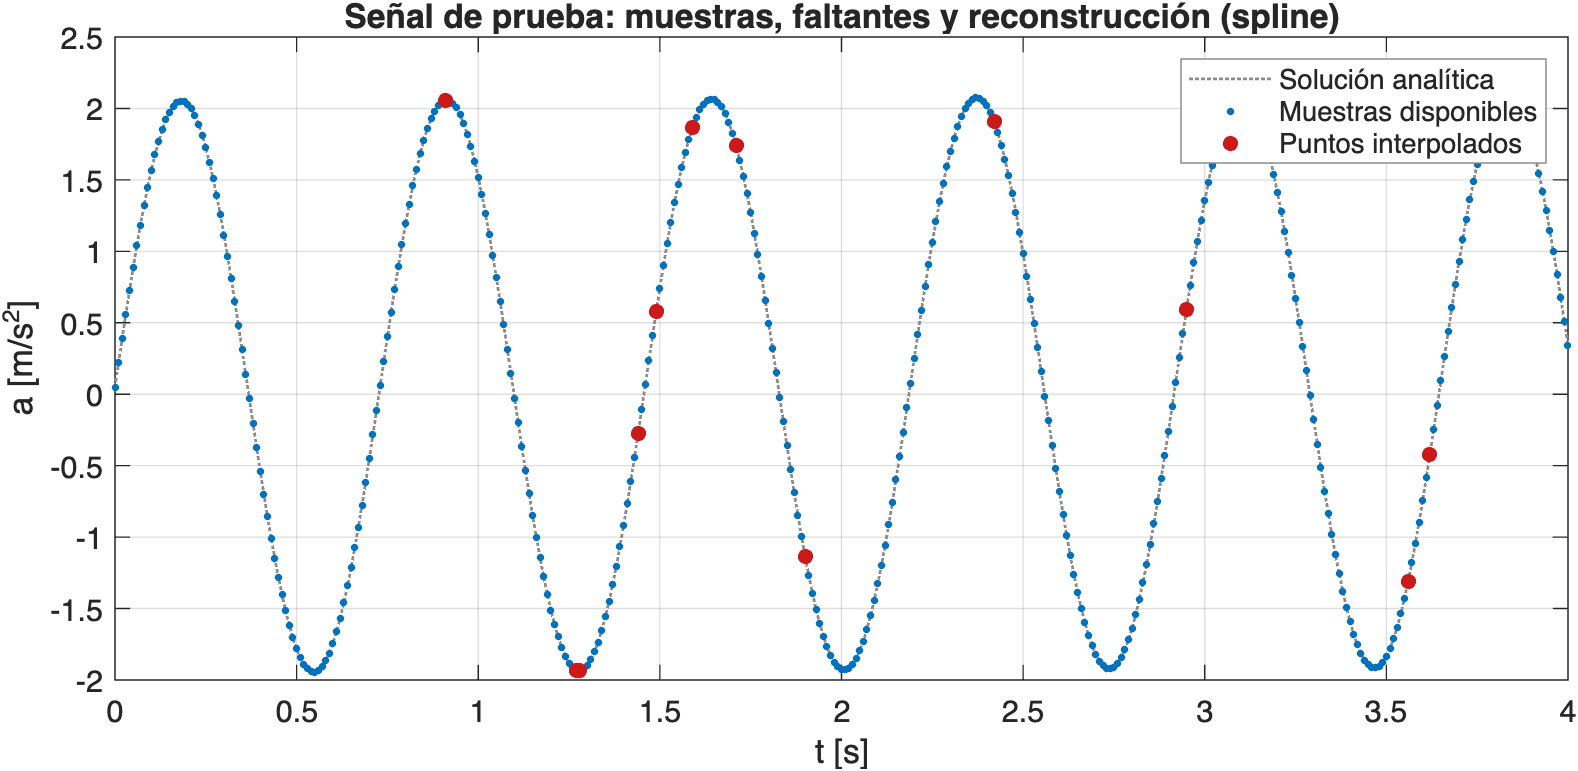
\includegraphics[width=0.9\linewidth]{f01_senal_prueba_faltantes.png}
\figurenote{Puntos azules: muestras disponibles. Puntos rojos: valores reconstruidos con el trazador cúbico natural. Línea punteada: solución analítica. Se muestran los primeros 4~s de 10~s.}
\end{figure}

\begin{table}[htbp]
\caption{Error de cada método contra la solución analítica}
\label{tab:validacion}
\centering\small
\begin{tabular}{@{}llccc@{}}
\toprule
Proceso & Método & Error & Orden observado & Orden teórico \\
\midrule
\multirow{3}{*}{Interpolación (máx.)} & Lineal & $1.48\times10^{-2}$ & -- & -- \\
 & Newton local cúbico & $5.48\times10^{-5}$ & -- & -- \\
 & Trazador natural & $3.01\times10^{-5}$ & -- & -- \\
\midrule
\multirow{4}{*}{Derivada ($h = 0.1$)} & Adelante & $5.00\times10^{-2}$ & 1.00 & 1 \\
 & Atrás & $5.00\times10^{-2}$ & 1.00 & 1 \\
 & Centrada & $3.32\times10^{-3}$ & 2.00 & 2 \\
 & Cinco puntos & $1.97\times10^{-5}$ & 3.99 & 4 \\
\midrule
\multirow{3}{*}{Integral ($n = 12$)} & Trapecio & $1.14\times10^{-2}$ & 2.00 & 2 \\
 & Simpson 1/3 & $5.26\times10^{-5}$ & 4.00 & 4 \\
 & Simpson 3/8 & $1.19\times10^{-4}$ & 4.01 & 4 \\
\midrule
\multirow{3}{*}{EDO, $x(t)$ ($h = 0.01$)} & Euler & $1.34\times10^{-2}$ & 1.11 & 1 \\
 & Heun & $1.42\times10^{-3}$ & 2.00 & 2 \\
 & RK4 & $1.93\times10^{-6}$ & 3.94 & 4 \\
\midrule
\multirow{2}{*}{Mínimos cuadrados} & Grados 1--4 vs.\ \texttt{polyfit} & $\le 3.3\times10^{-14}$ & -- & -- \\
 & Gauss con pivoteo vs.\ \texttt{A\textbackslash b} & $< 10^{-10}$ & -- & -- \\
\bottomrule
\end{tabular}
\figurenote{Resultados de \texttt{prueba\_metodos.m} ejecutado en \matlab{}. El orden observado es la pendiente de $\log E$ contra $\log h$ con cuatro valores de $h$ (tres para la EDO). En la EDO el orden se estimó con solo tres valores de $h$, por lo que el 1.11 de Euler, ligeramente mayor que el teórico, se encuentra dentro de la incertidumbre de esa estimación.}
\end{table}

\begin{figure}[htbp]
\caption{Convergencia de los métodos de derivación, integración y solución de la EDO}
\label{fig:convergencia}
\centering
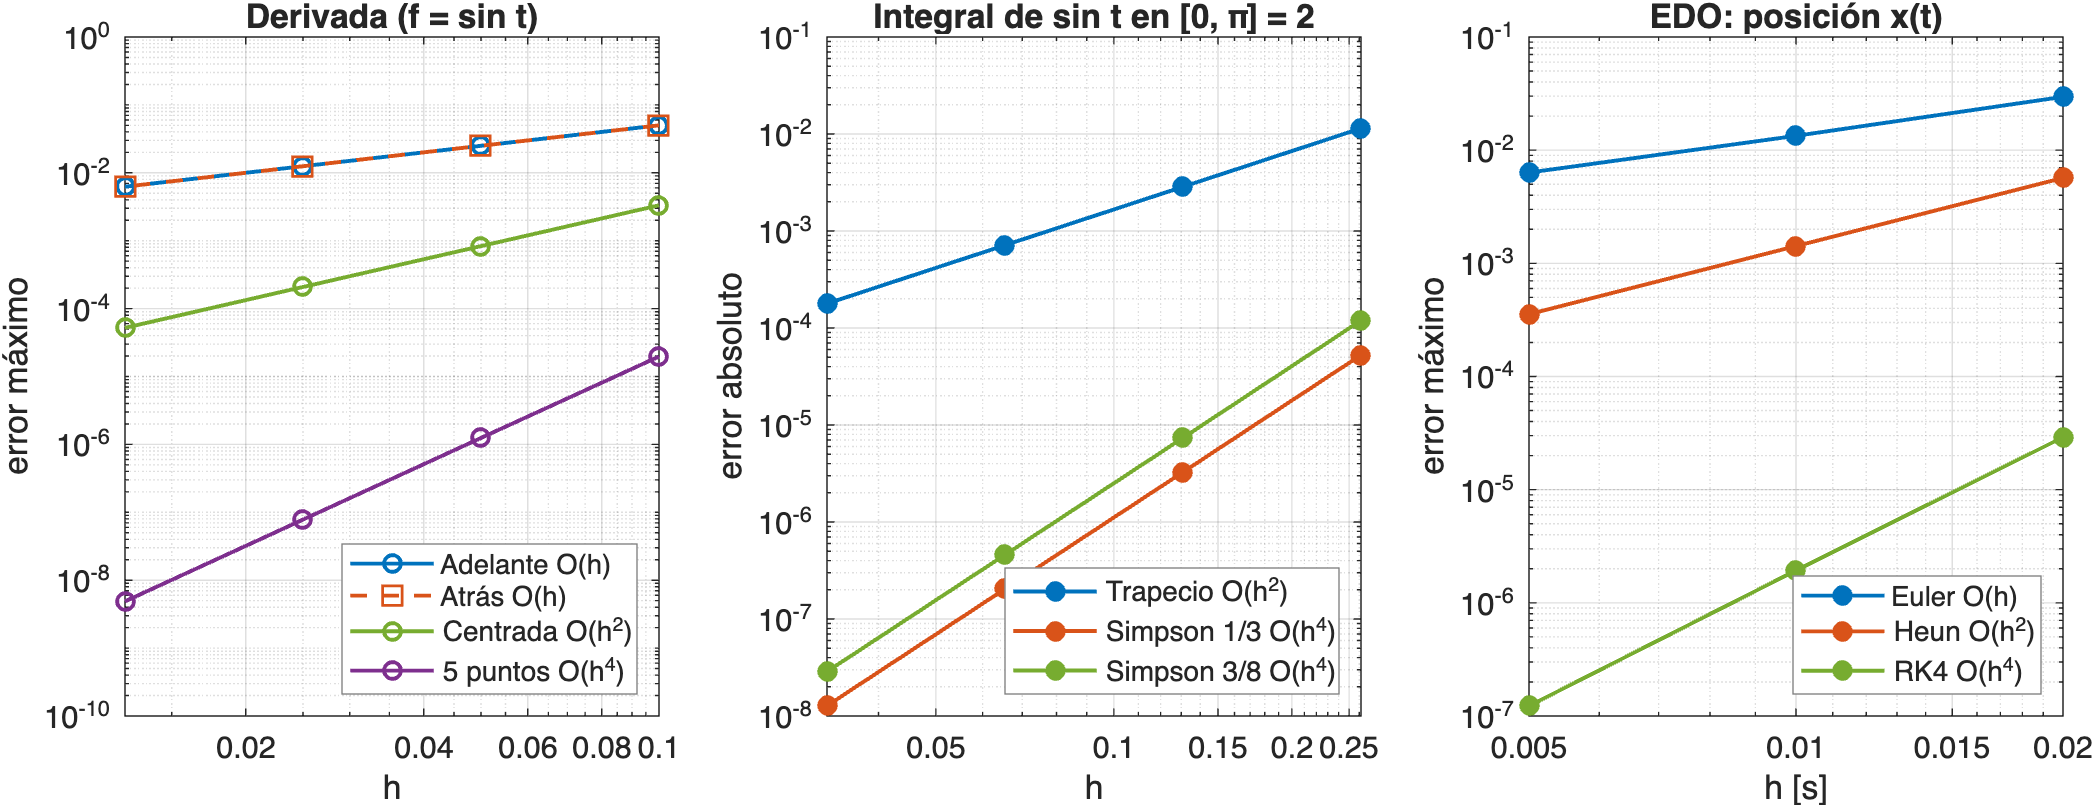
\includegraphics[width=\linewidth]{f02_convergencia.png}
\figurenote{Escalas logarítmicas. La pendiente de cada recta es el orden de convergencia. Las curvas de adelante y atrás coinciden porque ambas fórmulas tienen el mismo error máximo para $\sin t$.}
\end{figure}

\subsection{Duración y datos faltantes en las mediciones reales}

Las tres mediciones duraron entre 63.5 y 78.5~s, con un paso de muestreo de 0.01000~s y una variación (\textit{jitter}) de solo $1.7\times10^{-6}$~s (Tabla~\ref{tab:mediciones}). Ninguna tenía valores NaN ni huecos temporales. El filtro de Hampel detectó dos atípicos en el eje $z$ del cofre, ninguno en la cabina y cinco en el eje $x$ del manejo; cuatro de estos últimos alrededor de $t = 24.24$~s.

\subsection{Vibración del motor}

La Figura~\ref{fig:cofre} muestra la aceleración vertical sobre el cofre. El acercamiento de 0.4~s deja ver una oscilación regular con cerca de cuatro muestras por ciclo. El espectro (Figura~\ref{fig:espectro}) tiene un pico dominante en $f = 25.26$~Hz en los tres ejes; con la ecuación~\eqref{eq:rpm}, eso equivale a unas 758~rpm. En la cabina, media hora después, el pico apareció en 22.86~Hz (686~rpm), junto con su segundo armónico en 45.74~Hz, que es la componente dominante del eje $y$.

\begin{figure}[htbp]
\caption{Aceleración vertical medida sobre el cofre con el motor en ralentí}
\label{fig:cofre}
\centering
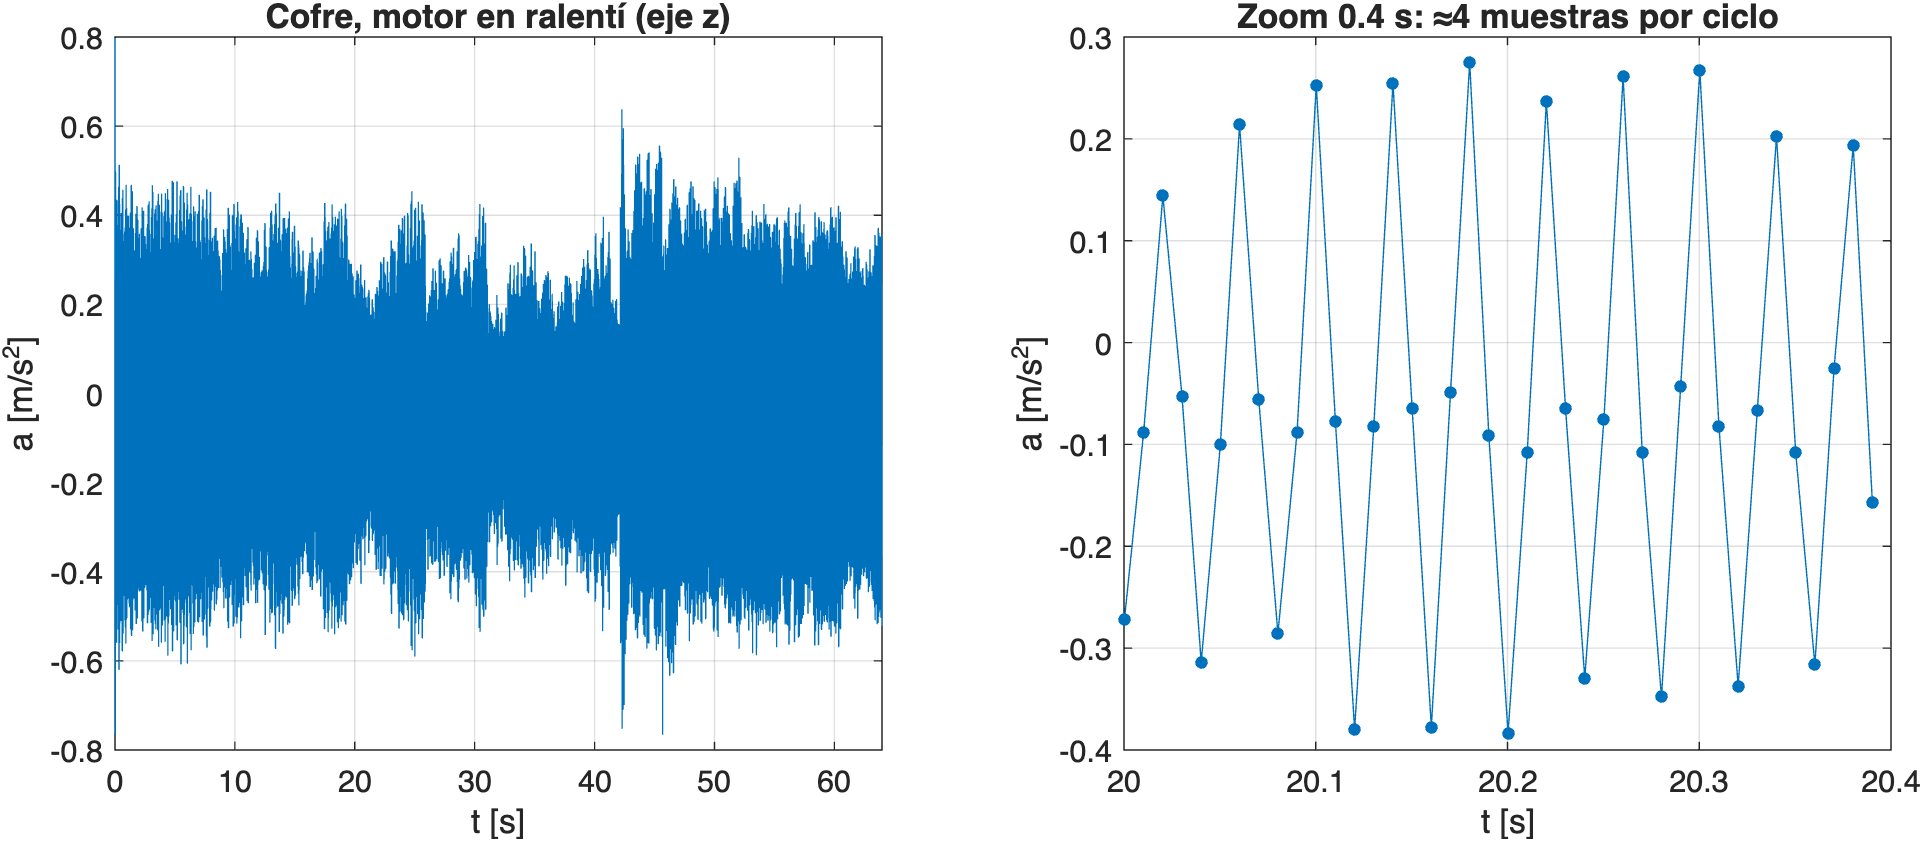
\includegraphics[width=\linewidth]{f03_cofre_senal_y_zoom.png}
\end{figure}

\begin{figure}[htbp]
\caption{Espectro de la vibración vertical en el cofre y en la cabina}
\label{fig:espectro}
\centering
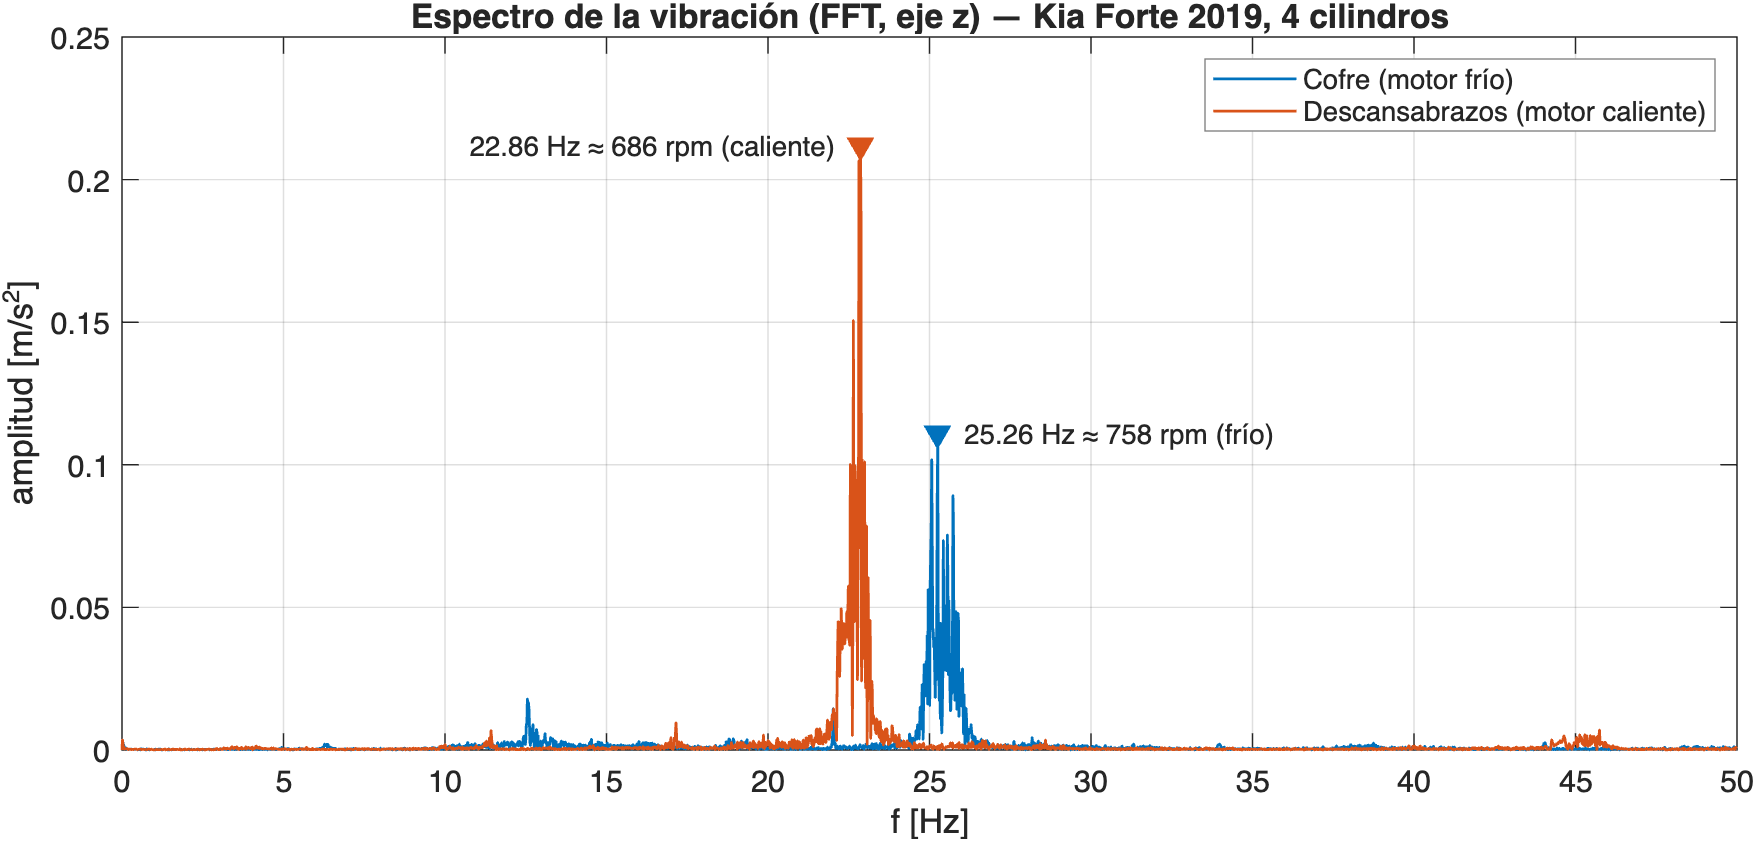
\includegraphics[width=0.95\linewidth]{f04_espectro_cofre_vs_cabina.png}
\figurenote{Espectro de amplitud de un lado calculado con FFT sobre toda la señal (resolución de 0.016~Hz).}
\end{figure}

Al analizar la señal del cofre en ventanas de 8~s, la frecuencia bajó de 25.75 a 25.00~Hz en el primer minuto (Tabla~\ref{tab:rpm}, Figura~\ref{fig:rpm}). Con el motor recién encendido, la unidad de control eleva el ralentí y lo reduce conforme el motor se calienta, que es lo que muestra la secuencia de mediciones. El espectro independiente de phyphox dio 22.65~Hz en la cabina, a 0.2~Hz del valor de esta aplicación. Esa diferencia es menor que la resolución de phyphox (0.39~Hz) y constituye una validación cruzada contra otro programa.

\begin{table}[htbp]
\caption{Frecuencia dominante y velocidad de ralentí estimada}
\label{tab:rpm}
\centering\small
\begin{tabular}{@{}llcc@{}}
\toprule
Hora & Medición & $f$ [Hz] & rpm ($=30f$) \\
\midrule
11:22 & Cofre, ventana 0--8~s (esta aplicación) & 25.75 & 773 \\
11:23 & Cofre, ventana 48--56~s (esta aplicación) & 25.00 & 750 \\
11:22--11:23 & Cofre, señal completa (esta aplicación) & 25.26 & 758 \\
11:26 & Cofre, \textit{Acceleration Spectrum} (phyphox) & 23.05 & 692 \\
11:54 & Cabina, señal completa (esta aplicación) & 22.86 & 686 \\
11:55 & Cabina, \textit{Acceleration Spectrum} (phyphox) & 22.65 & 680 \\
\bottomrule
\end{tabular}
\end{table}

\begin{figure}[htbp]
\caption{Velocidad de ralentí estimada en función del tiempo desde el arranque}
\label{fig:rpm}
\centering
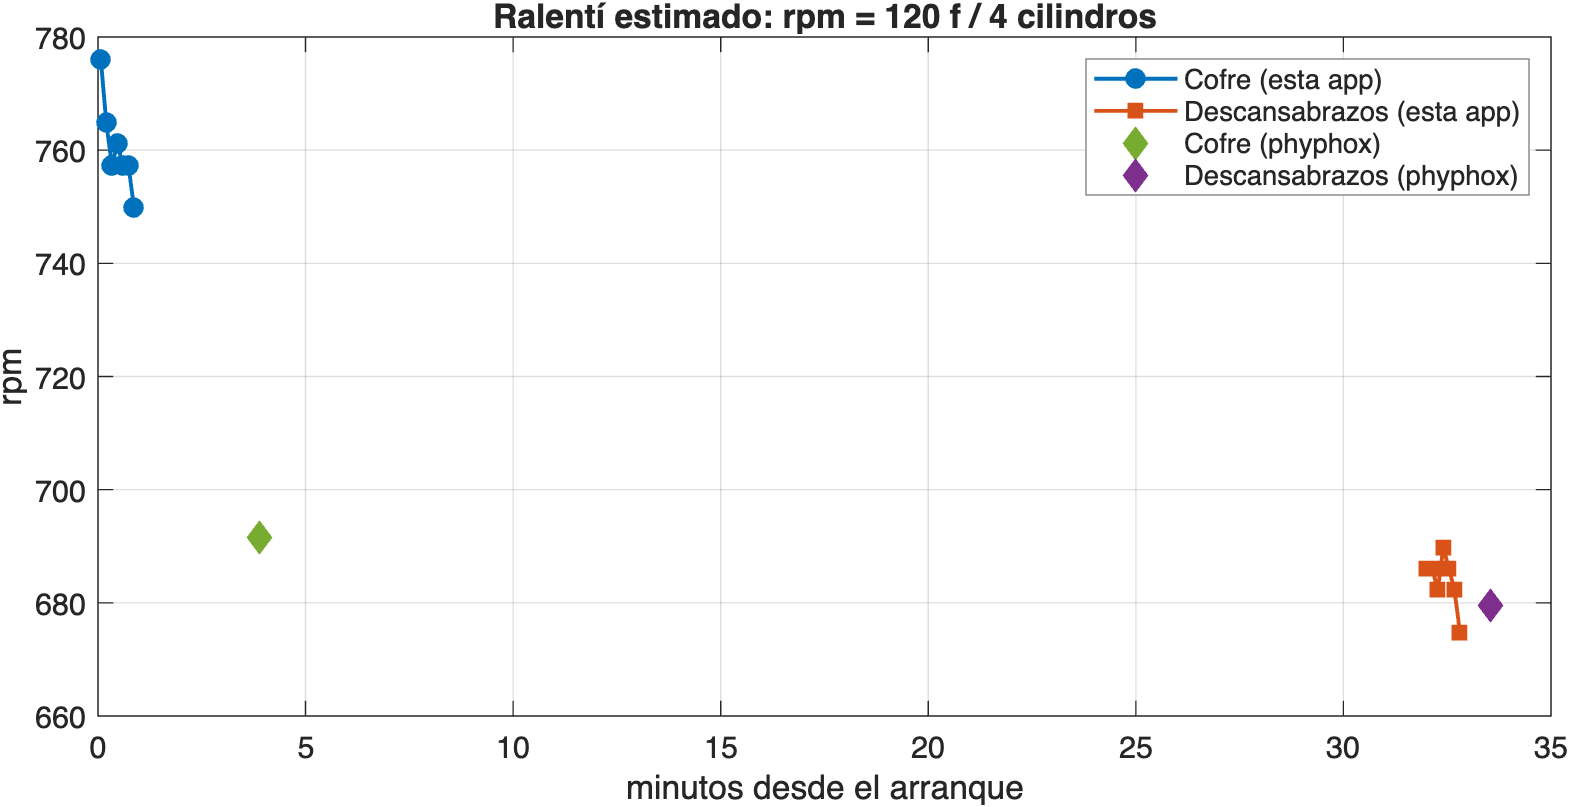
\includegraphics[width=0.85\linewidth]{f05_rpm_vs_tiempo.png}
\end{figure}

La amplitud no se comportó como se esperaba. La hipótesis era que la cabina vibraría menos que el cofre gracias a los soportes del motor, pero el valor RMS del eje $z$ fue de 0.430~m/s$^2$ en la cabina contra 0.289~m/s$^2$ en el cofre. La tapa plástica del descansabrazos es un panel ligero que puede amplificar la vibración, y además las dos mediciones se tomaron con el motor a velocidades distintas, de modo que con estos datos no se puede cuantificar el aislamiento de los soportes.

\subsection{Interpolación sobre datos reales}

La Tabla~\ref{tab:interp} y la Figura~\ref{fig:interp} comparan el error de reconstrucción al eliminar el 5\,\% de las muestras. En las tres mediciones reales el método lineal tuvo el menor error y el trazador cúbico el mayor, justo al revés que con la señal sintética.

\begin{table}[htbp]
\caption{Error RMS de interpolación con 5\,\% de muestras eliminadas [m/s$^2$]}
\label{tab:interp}
\centering\small
\begin{tabular}{@{}lccc@{}}
\toprule
Señal & Lineal & Newton local cúbico & Trazador natural \\
\midrule
Cofre, eje $z$ & \textbf{0.412} & 0.579 & 0.623 \\
Cabina, eje $z$ & \textbf{0.621} & 0.880 & 0.898 \\
Manejo, eje $x$ & \textbf{0.595} & 0.871 & 1.042 \\
Sintética (error máximo) & $1.5\times10^{-2}$ & $5.5\times10^{-5}$ & $\mathbf{3.0\times10^{-5}}$ \\
\bottomrule
\end{tabular}
\figurenote{Datos reales: semilla 1 de \texttt{prueba\_datos\_reales.m} en \matlab{}, entre 320 y 395 muestras evaluadas por señal. La Figura~\ref{fig:interp} usa el promedio de cinco semillas.}
\end{table}

\begin{figure}[htbp]
\caption{Error de interpolación por método y por señal}
\label{fig:interp}
\centering
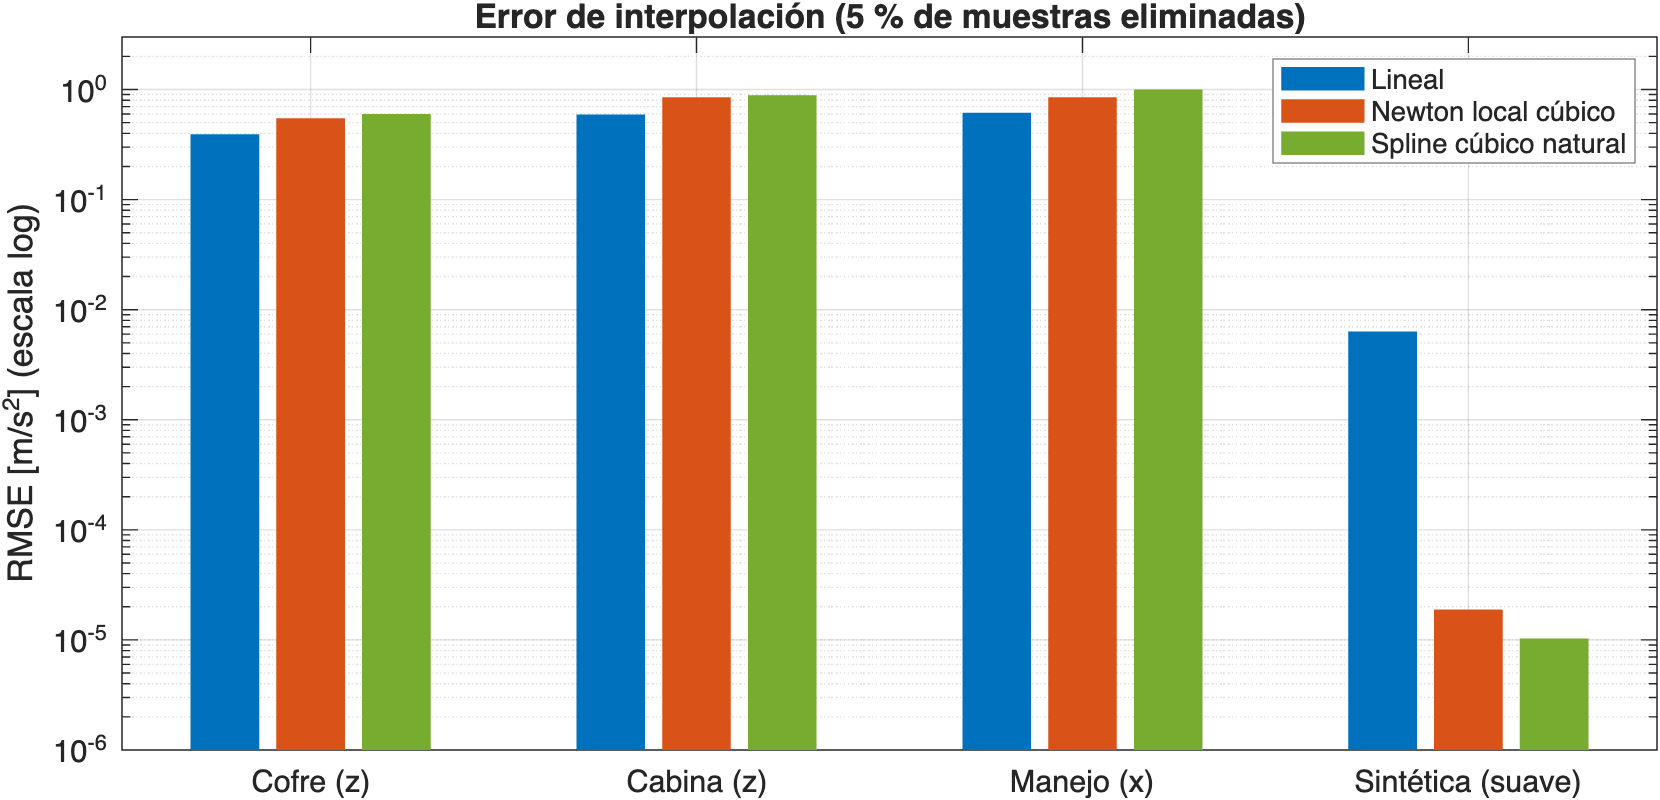
\includegraphics[width=0.9\linewidth]{f07_interpolacion_rmse.png}
\end{figure}

\subsection{Valores atípicos}

En la medición de manejo, en $t = 24.24$~s aparece una sola muestra de $-29.4$~m/s$^2$ (unas 3~$g$), mientras que las vecinas rondan 1~m/s$^2$ (Figura~\ref{fig:atipico}). El filtro de Hampel la detectó y la reconstruyó, y el pico máximo del eje $x$ bajó de 25.3 a 3.5~m/s$^2$. La primera versión del programa usaba un umbral global (mediana y MAD de toda la señal) y marcaba 106 «atípicos» en el eje $z$, que en realidad eran baches del camino. El criterio local de Hampel resolvió ese problema (bitácora, entrada 17).

\begin{figure}[htbp]
\caption{Pico aislado detectado con el filtro de Hampel en la medición de manejo}
\label{fig:atipico}
\centering
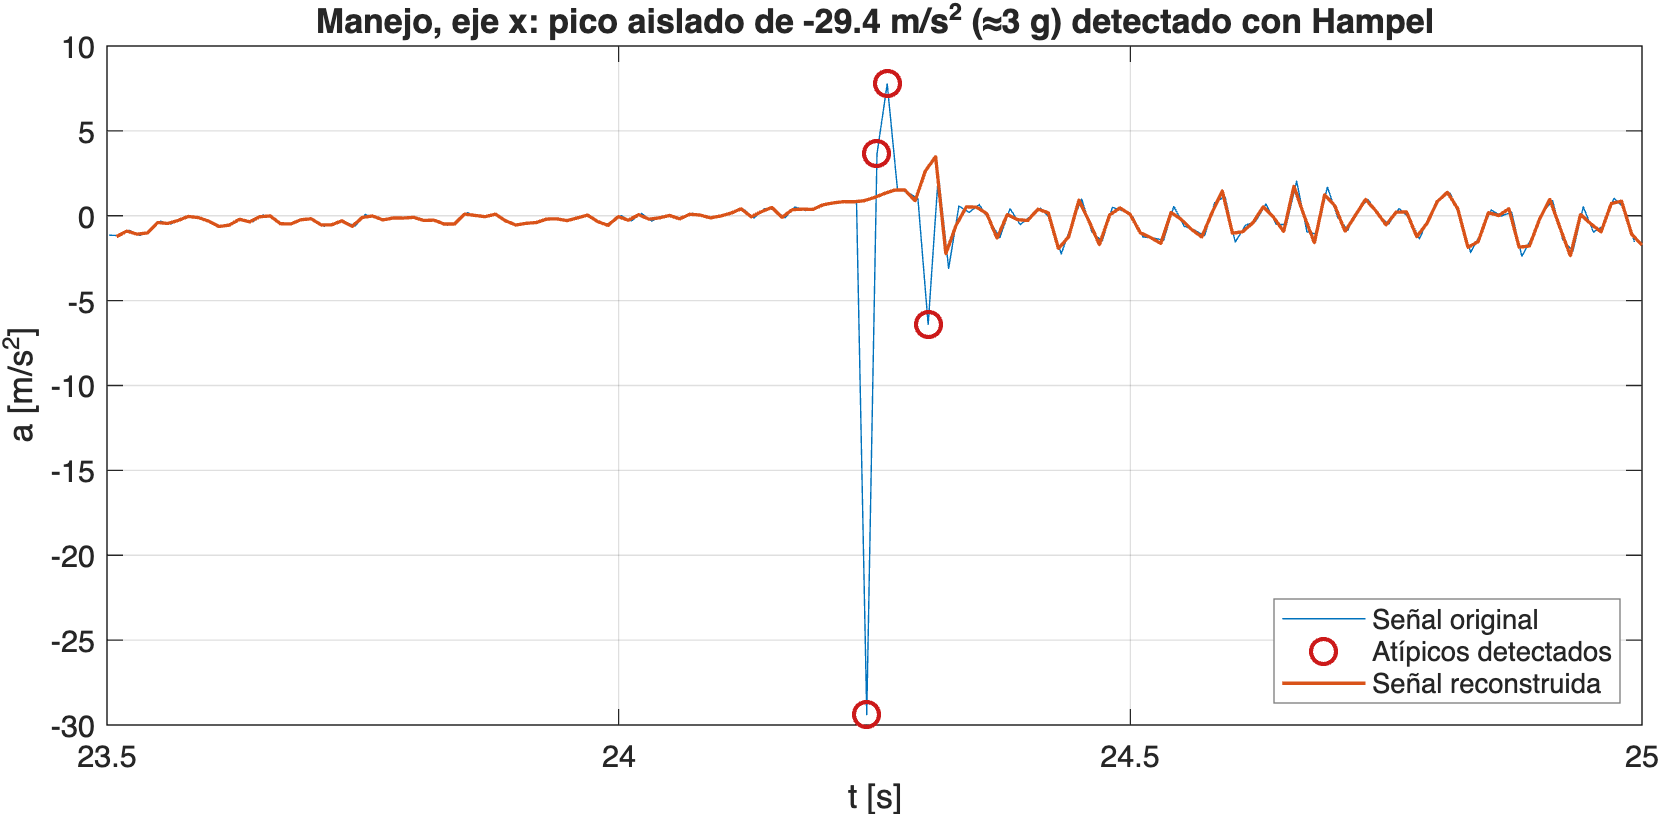
\includegraphics[width=0.9\linewidth]{f08_atipico_hampel.png}
\end{figure}

\subsection{Derivada de la señal}

Con la vibración del motor, $f/f_s = 0.253$ y $\theta = 1.587$~rad. Según la ecuación~\eqref{eq:factor}, la derivada centrada conserva solo el 63.0\,\% de la amplitud real del \textit{jerk}, la de cinco puntos el 84.3\,\% y la de adelante el 89.8\,\%, esta última con un desfase de 45.5$^\circ$ (Figura~\ref{fig:factor}). En la señal del cofre, el \textit{jerk} máximo fue de 109.3~m/s$^3$ con la fórmula centrada, 110.8 con la de cinco puntos y 93.6 con la de adelante.

\begin{figure}[htbp]
\caption{Fracción de la amplitud que conserva cada fórmula de derivación}
\label{fig:factor}
\centering
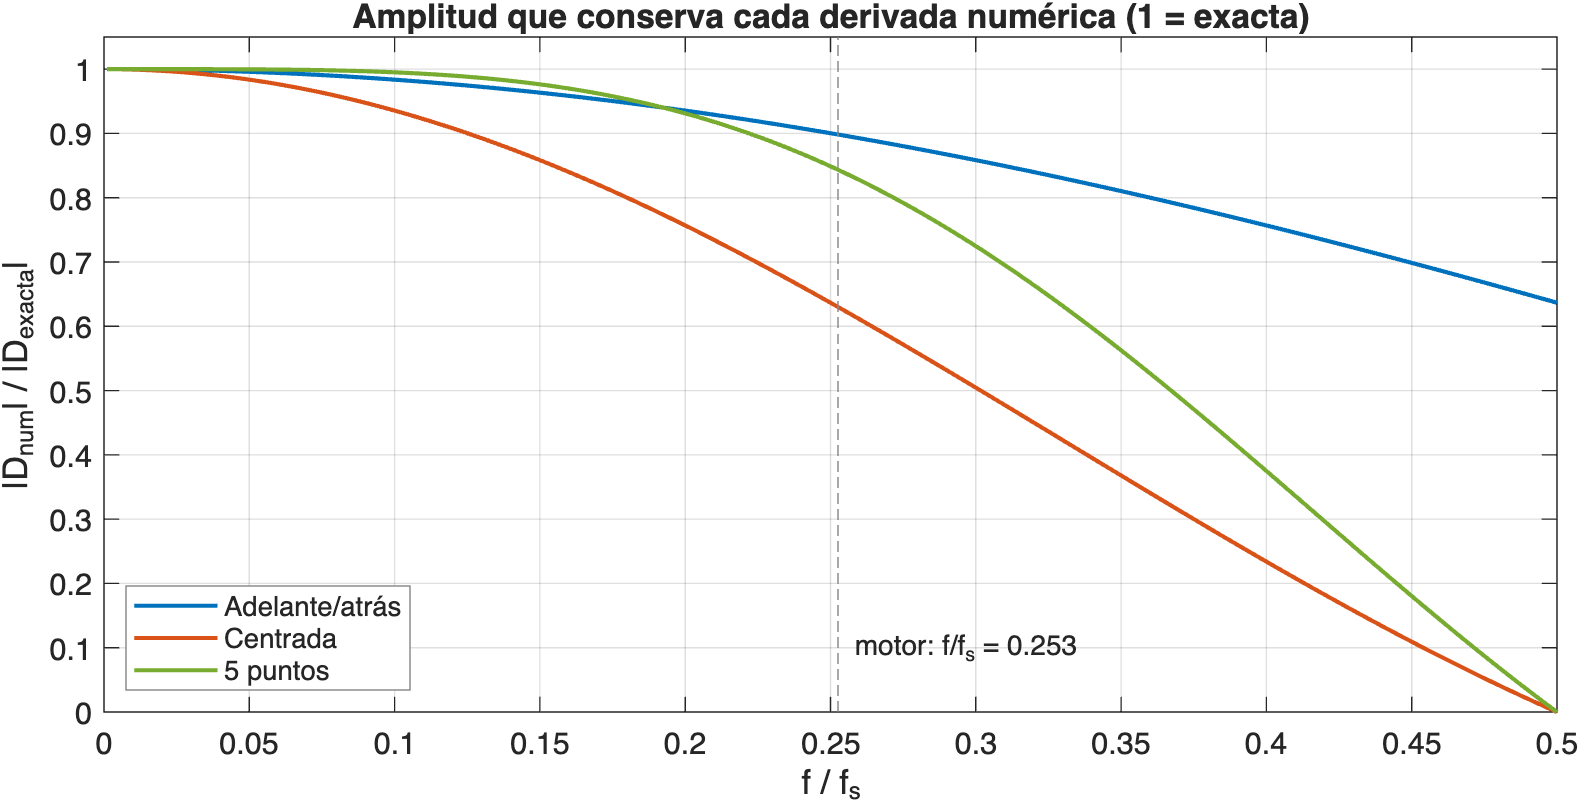
\includegraphics[width=0.85\linewidth]{f09_factor_derivadas.png}
\figurenote{La línea discontinua marca la frecuencia del motor en ralentí (25.26~Hz) con $f_s = 100$~Hz.}
\end{figure}

\subsection{Integral, ecuación diferencial y deriva}

Con el vehículo estacionado la velocidad y el desplazamiento reales son prácticamente nulos, lo que da una referencia exacta para evaluar la integración. Sin corrección, la integral de la aceleración del cofre indica que el vehículo alcanzó 4.09~m/s y se desplazó 127~m (Tabla~\ref{tab:deriva}, Figura~\ref{fig:deriva}). El sesgo medido fue $\hat b = -0.0639$~m/s$^2$; la ecuación~\eqref{eq:deriva} predice $\Delta v = 4.09$~m/s y $\Delta x = 130.8$~m, valores que concuerdan con lo observado, así que el error se debe casi por completo al sesgo. Restar la tendencia de grado 1 redujo el desplazamiento final a 0.31~m, más de 400 veces menos.

\begin{table}[htbp]
\caption{Velocidad y desplazamiento integrados con RK4 según la corrección de deriva}
\label{tab:deriva}
\centering\small
\begin{tabular}{@{}llccc@{}}
\toprule
Medición & Corrección & $v(T)$ [m/s] & $|v|_{\max}$ [m/s] & $x(T)$ [m] \\
\midrule
\multirow{3}{*}{Cofre (estacionado)} & Ninguna & $-4.094$ & 4.094 & $-127.23$ \\
 & Sesgo constante (MC grado 0) & $-0.006$ & 0.088 & 3.54 \\
 & Tendencia MC grado 1 & $-0.006$ & 0.031 & $\mathbf{-0.31}$ \\
\midrule
\multirow{3}{*}{Cabina (estacionado)} & Ninguna & $-5.246$ & 5.246 & $-163.08$ \\
 & Sesgo constante & 0.001 & 0.093 & 3.60 \\
 & Tendencia MC grado 1 & 0.001 & 0.020 & $\mathbf{0.12}$ \\
\midrule
\multirow{3}{*}{Manejo, eje $x$} & Ninguna & 4.446 & 5.335 & 180.25 \\
 & Sesgo constante & 0.002 & 2.758 & 5.77 \\
 & Tendencia MC grado 1 & 0.002 & 2.654 & 0.18 \\
\bottomrule
\end{tabular}
\figurenote{En el manejo se activó el filtro de Hampel. En ese caso la posición no representa el recorrido real del vehículo, porque el eje del teléfono no estaba alineado con la dirección de avance.}
\end{table}

\begin{figure}[htbp]
\caption{Velocidad y posición integradas del vehículo estacionado (cofre, eje $z$)}
\label{fig:deriva}
\centering
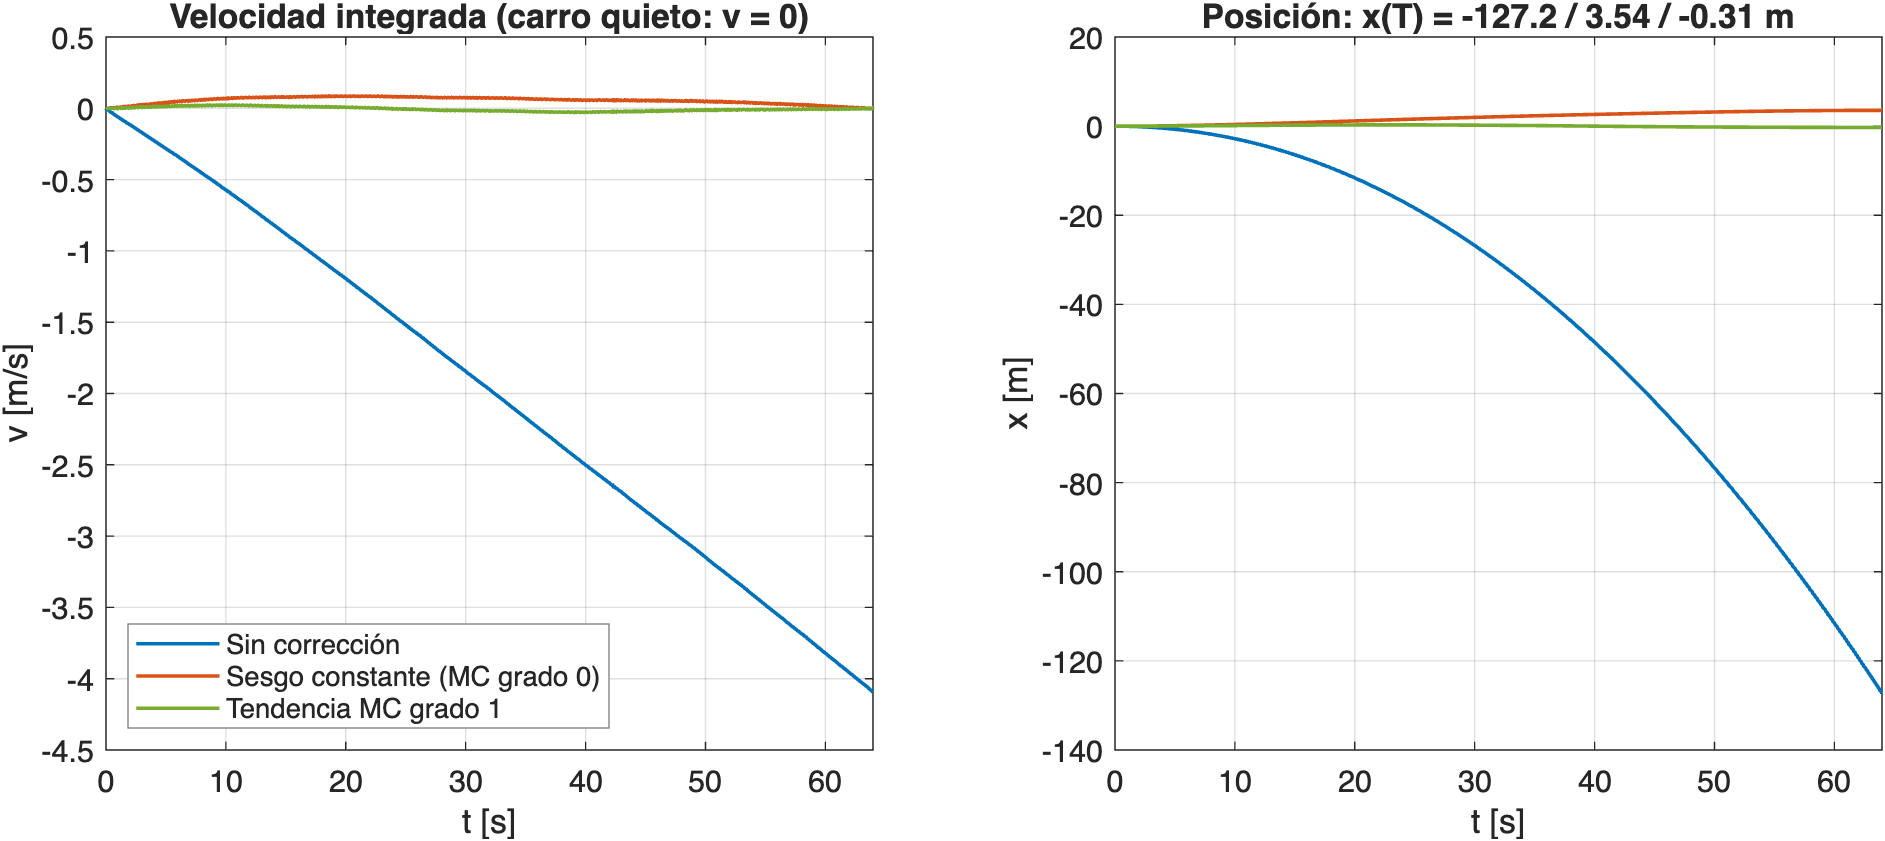
\includegraphics[width=\linewidth]{f06_drift_velocidad_posicion.png}
\end{figure}

Las tres reglas de integración aplicadas a la señal real sin corregir dieron valores casi iguales en el cofre: $-4.288$ (trapecio), $-4.282$ (Simpson 1/3) y $-4.294$~m/s (Simpson 3/8), con diferencias menores al 0.15\,\%. En la ecuación diferencial, Heun y la integral doble con \texttt{cumtrapz} difirieron solo $5\times10^{-5}$~m. Es lo esperado, porque cuando $\mathbf{f}$ no depende del estado Heun se reduce a la regla del trapecio. RK4 y Euler difirieron de esa referencia en 0.03 y 0.30~m, respectivamente.

La Figura~\ref{fig:manejo} presenta la velocidad del eje $x$ del teléfono durante el manejo. Sin corrección la velocidad termina en 16~km/h; con el sesgo constante regresa a cero, aunque toma valores negativos porque el eje del teléfono no coincidía con la dirección de avance del vehículo.

\begin{figure}[htbp]
\caption{Velocidad integrada en el eje $x$ del teléfono durante el manejo}
\label{fig:manejo}
\centering
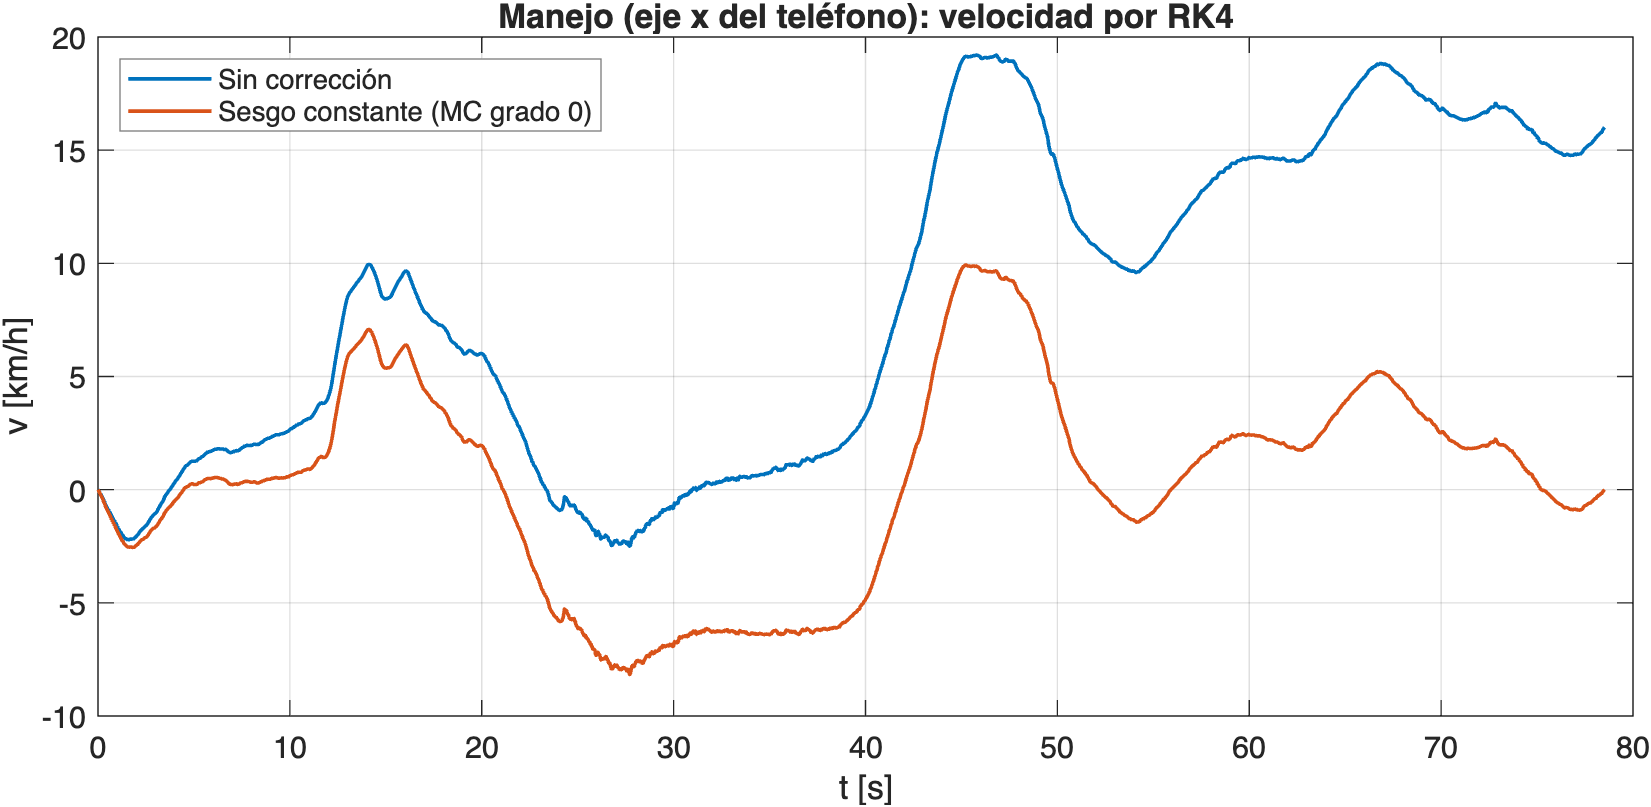
\includegraphics[width=0.9\linewidth]{f10_manejo_velocidad.png}
\end{figure}

\subsection{Línea de tendencia por mínimos cuadrados}

Las tendencias de grado 1 a 3 sobre la señal de manejo tienen coeficientes de determinación muy bajos, de $R^2 = 0.0000$, $0.0023$ y $0.0073$ (Figura~\ref{fig:tendencia}). Esto es lo correcto: la tendencia no pretende explicar la vibración, que oscila alrededor de cero, sino separar el sesgo y la deriva lenta del sensor. Gracias a la variable escalada, el número de condición de la matriz normal fue de 1.0, 7.6, 35.8 y 211.5 para los grados 1 a 4. Sin escalamiento, la matriz de Vandermonde con $t$ entre 0 y 80~s tendría números de condición de muchos órdenes de magnitud más.

\begin{figure}[htbp]
\caption{Líneas de tendencia por mínimos cuadrados sobre la señal de manejo}
\label{fig:tendencia}
\centering
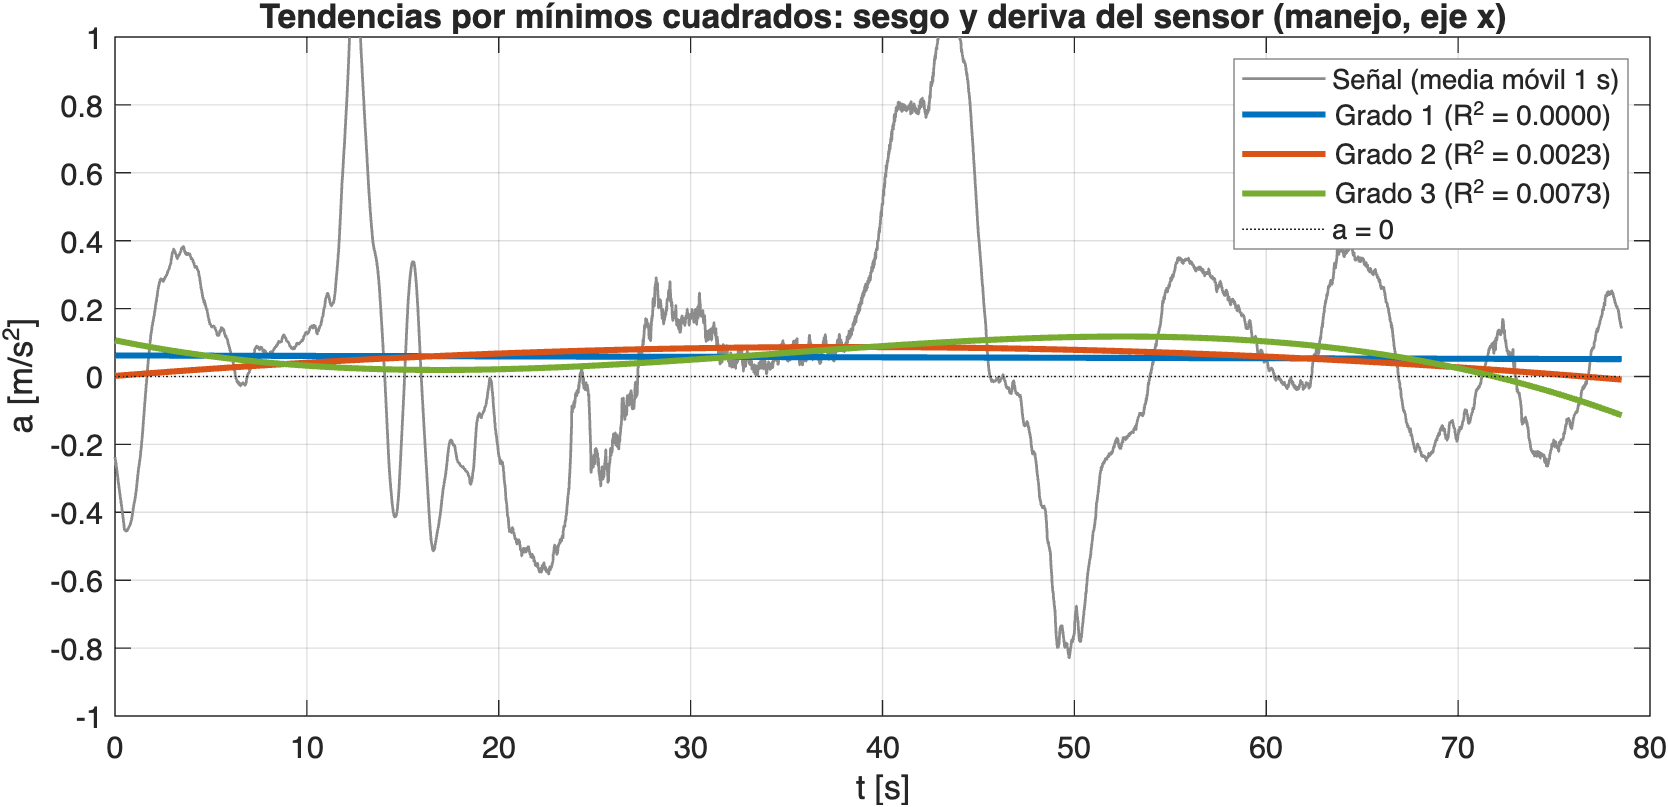
\includegraphics[width=0.9\linewidth]{f11_tendencia_mc.png}
\end{figure}

\subsection{Funcionamiento de la aplicación}

Las Figuras~\ref{fig:app} a~\ref{fig:foto} muestran la aplicación en funcionamiento con los datos reales: el panel de control, la reproducción en tiempo real durante una grabación, la validación de métodos y los archivos exportados.

\begin{figure}[htbp]
\caption{Interfaz del analizador con la medición del cofre}
\label{fig:app}
\centering
\captura{app_general.png}{\linewidth}{captura de la ventana completa con \texttt{motor\_ralenti\_cofre.csv}, eje $z$, tema claro}
\figurenote{Izquierda: panel de control. Arriba: datos originales. Centro: señal procesada. Abajo: resultados.}
\end{figure}

\begin{figure}[htbp]
\caption{Monitor en tiempo real durante una grabación}
\label{fig:tiemporeal}
\centering
\captura{app_tiempo_real.png}{\linewidth}{captura de la pestaña \textit{Tiempo real} con la grabación activa (segmento en rojo e indicador encendido)}
\end{figure}

\begin{figure}[htbp]
\caption{Pestaña de validación de métodos con datos reales}
\label{fig:appvalidacion}
\centering
\captura{app_validacion.png}{\linewidth}{captura de la pestaña \textit{Validación de métodos} después de pulsar \textit{Comparar todos los métodos}}
\end{figure}

\begin{figure}[htbp]
\caption{Exportación de resultados con nombre definido por el usuario}
\label{fig:exportacion}
\centering
\captura{app_exportacion.png}{0.48\linewidth}{diálogo de guardado con el nombre escrito}\hfill
\captura{app_archivos.png}{0.48\linewidth}{carpeta con el .xlsx y los PNG claro/oscuro exportados}
\end{figure}

\begin{figure}[htbp]
\caption{Fotografía de la aplicación en funcionamiento}
\label{fig:foto}
\centering
\captura{foto_app_funcionando.jpg}{0.8\linewidth}{fotografía de la computadora ejecutando la aplicación}
\end{figure}

\section{Análisis de resultados}
\label{sec:analisis}

\subsection{Efectividad de los métodos en el algoritmo integrador}

La Tabla~\ref{tab:efectividad} resume qué método resultó más efectivo en cada proceso y la evidencia que lo respalda. La conclusión general es que el orden de convergencia no basta para decidir. Con datos reales manda la relación entre la frecuencia de la señal y la de muestreo, junto con el ruido y el sesgo del sensor.

\begin{longtable}{@{}p{2.4cm}p{3.2cm}p{4.3cm}p{4.3cm}@{}}
\caption{Método más efectivo en cada proceso}\label{tab:efectividad}\\
\toprule
Proceso & Método elegido & Evidencia & Justificación \\
\midrule
\endfirsthead
\toprule
Proceso & Método elegido & Evidencia & Justificación \\
\midrule
\endhead
\bottomrule
\endfoot
Atípicos & Hampel local & 106 falsos positivos con umbral global; 1 a 5 por eje con Hampel & La señal no es estacionaria: un umbral global confunde los baches reales con errores \\
Interpolación (datos reales) & Lineal & RMSE de 0.41 a 0.62 contra 0.62 a 1.04 del trazador & Con cerca de 4 muestras por ciclo, los polinomios cúbicos sobreoscilan entre muestras; la lineal queda acotada por sus vecinos \\
Interpolación (señal suave) & Trazador natural & $3.0\times10^{-5}$ contra $1.5\times10^{-2}$ de la lineal & Con más de 70 muestras por ciclo, la curvatura continua del trazador reproduce bien la señal \\
Derivada & Cinco puntos & Orden 3.99; conserva el 84\,\% de la amplitud a 25~Hz contra el 63\,\% de la centrada & Menor error de truncamiento y menor atenuación a la frecuencia del motor \\
Integral & Simpson 1/3 & Error de $5.3\times10^{-5}$ contra $1.1\times10^{-2}$ del trapecio ($n = 12$) & Orden 4 con el mismo número de evaluaciones; con datos reales las tres reglas difieren menos del 0.15\,\% \\
EDO & RK4 & Error en $x$ de $1.9\times10^{-6}$ contra $1.3\times10^{-2}$ de Euler & Orden 4. Con datos medidos su ventaja queda por debajo del error por sesgo \\
Deriva & MC grado 1 & Desplazamiento falso de 127~m reducido a 0.31~m & Modela el sesgo y su deriva lenta; el grado 0 basta cuando el sistema inicia y termina en reposo \\
Frecuencia & FFT de la señal completa & 22.86 contra 22.65~Hz de phyphox & Mayor resolución (0.016~Hz) que la ventana de 2.56~s de phyphox (0.39~Hz) \\
\end{longtable}

\subsection{Interpolación: por qué la lineal ganó con datos reales}

La señal sintética oscila a 1.37~Hz y se muestrea a 100~Hz: unas 73 muestras por ciclo. Entre dos muestras la función es casi un arco de parábola, de modo que un polinomio cúbico la reproduce mejor que una recta. La vibración del motor, en cambio, tiene unas cuatro muestras por ciclo y ruido de medición de alrededor de 0.05~m/s$^2$. El trazador y el polinomio de Newton pasan exactamente por puntos ruidosos y muy separados en fase, y entre ellos generan curvaturas que la señal real no tiene. Por eso su error máximo fue hasta 1.6 veces el de la interpolación lineal (1.59 contra 1.02~m/s$^2$ en el cofre). En la aplicación se dejan los tres métodos disponibles: el usuario puede comprobar en la pestaña de validación cuál conviene para su señal.

\subsection{Derivada: orden contra atenuación}

Con $h$ fijo, aumentar el orden no siempre se traduce en menor error. La fórmula de adelante conserva más amplitud que la centrada a 25~Hz (89.8 contra 63.0\,\%), pero desplaza la señal medio paso y su error de truncamiento es de primer orden, como se ve en la Figura~\ref{fig:convergencia}. La de cinco puntos combina el mayor orden con una atenuación moderada, aunque usa cinco muestras y amplifica más el ruido: la suma de los valores absolutos de sus pesos es $18/12 = 1.5$ veces la de la centrada. Para estimar el \textit{jerk} del motor se recomienda la de cinco puntos. Si la señal fuera muy ruidosa, convendría filtrarla antes de derivar.

\subsection{Integración y ecuación diferencial: el error dominante es el sesgo}

En la validación analítica, la jerarquía teórica se cumple: Simpson supera al trapecio por más de dos órdenes de magnitud y RK4 a Euler por casi cuatro. Con los datos del vehículo estacionado, en cambio, la diferencia entre métodos (unos 0.3~m entre Euler y RK4) es despreciable frente al error de 127~m que produce un sesgo de 0.064~m/s$^2$. La ecuación~\eqref{eq:deriva} reproduce ese error con menos del 3\,\% de diferencia. Por eso la corrección por mínimos cuadrados fue el paso con mayor impacto en la calidad del resultado, por encima de la elección del integrador. El grado 1 dio mejores resultados que el 0 en las mediciones estacionadas porque el sesgo del sensor cambió lentamente durante el minuto de medición.

\subsection{Limitaciones}

\begin{itemize}
  \item \textbf{Frecuencia de muestreo.} A 100~Hz solo se observan vibraciones por debajo de 50~Hz; en un motor de cuatro cilindros eso equivale a unas 1500~rpm. Durante el manejo aparecieron componentes de hasta 49~Hz, cerca del límite de Nyquist.
  \item \textbf{Orientación.} En el manejo el teléfono no estaba alineado con el vehículo, así que la velocidad del eje $x$ mezcla movimiento longitudinal y lateral. Corregirlo requeriría fusionar el acelerómetro con el giroscopio.
  \item \textbf{Comparación cofre--cabina.} Las mediciones no fueron simultáneas y el motor giraba a velocidades distintas, por lo que no permiten cuantificar el aislamiento de los soportes.
  \item \textbf{Pérdida simulada.} El error de interpolación se midió sobre huecos generados artificialmente. Con pérdidas reales más largas el error crecería.
\end{itemize}

\section{Conclusiones}

Se construyó en \matlab{} una aplicación con interfaz gráfica que integra los métodos numéricos del curso para analizar la vibración real de un automóvil medida con el acelerómetro de un teléfono. La aplicación calcula la duración de la señal, detecta e interpola datos faltantes, obtiene la derivada y la integral, resuelve la ecuación diferencial del movimiento y ajusta líneas de tendencia por mínimos cuadrados. Ofrece menús para elegir algoritmos y parámetros, gráficas de los datos originales y procesados, indicadores numéricos, reproducción en tiempo real con grabación controlada por el usuario y exportación con nombre de archivo definido por él. Con esto se cubren todos los requisitos del proyecto.

Los métodos se programaron sin usar las funciones equivalentes de \matlab{} y se validaron contra una solución analítica. Los órdenes de convergencia observados coinciden con los teóricos, y la diferencia frente a \texttt{interp1}, \texttt{gradient}, \texttt{trapz} y \texttt{polyfit} es del orden del redondeo de máquina cuando el método es equivalente.

Con las mediciones reales, la aplicación identificó la frecuencia de encendido del motor (25.26~Hz, unas 758~rpm con el motor frío) y registró su descenso a 22.86~Hz (686~rpm) al calentarse, en concordancia con la medición independiente de phyphox. También mostró que integrar la aceleración sin corregir el sesgo produce un desplazamiento falso de más de 100~m en un vehículo estacionado y que la tendencia por mínimos cuadrados lo reduce a centímetros.

La principal lección del análisis es que el método más efectivo depende de la señal. Con una señal suave y bien muestreada se cumple la jerarquía teórica: trazador antes que lineal, cinco puntos antes que centrada, Simpson antes que trapecio y RK4 antes que Euler. Con la vibración real, a unas cuatro muestras por ciclo, la interpolación lineal superó a las cúbicas, y el error de integración lo dominó el sesgo del sensor, no el orden del integrador. Elegir un algoritmo de forma justificada exige comparar los métodos con los datos del problema, y la aplicación incluye una pestaña para hacerlo.

Como trabajo futuro se proponen tres mejoras: medir simultáneamente en el cofre y en la cabina para cuantificar el aislamiento de los soportes del motor; usar un sensor externo con mayor frecuencia de muestreo para observar los armónicos superiores; y fusionar el acelerómetro con el giroscopio para estimar la velocidad del vehículo independientemente de la orientación del teléfono.


\clearpage
\printbibliography[title=Referencias]

\clearpage
\appendix
\section{Bitácora de desarrollo}
\label{app:bitacora}

Registro de las decisiones de diseño, los errores encontrados durante el desarrollo y sus soluciones, entre el 21 y el 25 de noviembre de 2026. La versión actualizada está en \texttt{App/bitacora.md}.

{\scriptsize
\setlength{\tabcolsep}{3pt}
\begin{longtable}{@{}p{0.5cm}p{1.6cm}p{3.3cm}p{3.1cm}p{3.6cm}p{2.4cm}@{}}
\caption{Bitácora de errores y soluciones}\label{tab:bitacora}\\
\toprule
\# & Etapa & Problema o decisión & Causa & Solución & Verificación \\
\midrule
\endfirsthead
\toprule
\# & Etapa & Problema o decisión & Causa & Solución & Verificación \\
\midrule
\endhead
\endfoot
1 & Diseño & Separar la matemática de la interfaz & Una GUI no se puede probar automáticamente & Motor \texttt{nm\_procesar} + funciones \texttt{nm\_*}; la GUI solo llama y grafica & \texttt{pruebas/prueba\_motor.m} corre sin interfaz \\ \midrule
2 & Integración & Simpson 3/8 no era exacto para cúbicas con 7 intervalos & El residuo de 1 intervalo se integraba con trapecio (O(h\textsuperscript{2})) & Residuo de 4 intervalos $\rightarrow$ 2 $\times$ Simpson 1/3 (O(h\textsuperscript{4})) & Exacto para x³ con 3 a 11 intervalos \\ \midrule
3 & Validación EDO & Orden de convergencia "negativo" en Heun y RK4 & Se medía el error solo en t = T, donde 1 − cos(wT) = 0 por coincidencia & Medir el error máximo en toda la trayectoria x(t) & Órdenes 1.11 / 2.00 / 3.94 \\ \midrule
4 & Validación integral & Trapecio parecía más exacto que Simpson & La señal de prueba tenía un número entero de periodos (15 ciclos): el trapecio es superconvergente para funciones periódicas en periodos completos & f = 1.37 Hz (13.7 ciclos) & Simpson 1.4e-7 vs trapecio 1.9e-4 \\ \midrule
5 & Código & \texttt{w} indefinida en \texttt{nm\_senal\_prueba} & Al editar, dos sentencias quedaron en la misma línea detrás de un comentario \texttt{\%} & Separar las líneas & Pruebas pasan \\ \midrule
6 & Validación & Newton local comparado contra \texttt{interp1('pchip')} & pchip es Hermite con preservación de forma, no el mismo polinomio & Marcar "sin equivalente directo" y validar solo contra la solución analítica & Error 1.8e-5 vs analítica \\ \midrule
7 & GUI & Eje derecho de \texttt{yyaxis} persistía al cambiar de vista & \texttt{cla} no elimina el segundo eje Y & \texttt{cla(ax,'reset')} & Revisión de código (pendiente de prueba en MATLAB) \\ \midrule
8 & GUI & Etiquetas de la gráfica de errores sin espacio & \texttt{strcat} elimina espacios finales en argumentos \texttt{char} & Concatenar con \texttt{cellfun} & Revisión de código \\ \midrule
9 & GUI & Posible error al cambiar de archivo con distinto número de ejes & \texttt{Items} e \texttt{ItemsData} del menú con longitudes distintas & \texttt{fijarItems}: vaciar \texttt{ItemsData}, asignar \texttt{Items} y luego \texttt{ItemsData} & Revisión de código \\ \midrule
10 & Física & Velocidad final de 2.09 m/s al integrar la aceleración en reposo & Sesgo y deriva térmica del acelerómetro integrados en el tiempo (drift) & Restar la tendencia por mínimos cuadrados antes de integrar & v(T) $\approx$ 0 m/s \\ \midrule
11 & Mínimos cuadrados & Error al ajustar grado 0 (media) & En la sustitución hacia atrás, \texttt{x(i+1:n)} de un escalar da un vector 1$\times$0 y el producto no es conforme & Sumatoria explícita con ciclo \texttt{for} & MC grado 0 = media (prueba) \\ \midrule
12 & Diseño / física & Restar la tendencia lineal distorsiona el ensayo arranque–frenado del carro & En ese ensayo la aceleración es positiva al inicio y negativa al final; la recta de MC tiene pendiente real que no es drift & 4 opciones de corrección: ninguna, sesgo constante (MC grado 0), tendencia MC, reposo inicial. Para inicio y fin en reposo se usa el sesgo constante & Comparación en \texttt{prueba\_motor.m} \\ \midrule
13 & Datos reales & Los datos del iPhone casi no tienen huecos, entonces la interpolación no se podía evaluar & Con señal real no se conoce el valor verdadero de un dato faltante & \texttt{nm\_simular\_perdida}: elimina en ráfagas un \% de muestras reales y compara el interpolante contra el valor verdadero (RMSE) & Lineal 0.34, Newton 0.12, spline 0.14 m/s\textsuperscript{2} (ejemplo) \\ \midrule
14 & GUI & Riesgo: \texttt{exportgraphics} sobre gráficas de pestañas no visibles & Las pestañas ocultas no se dibujan & Seleccionar la pestaña antes de exportar y restaurarla después & \texttt{prueba\_gui.m} \\ \midrule
15 & Pruebas & Una prueba manual de la GUI no detecta todos los errores & Muchas combinaciones de menús & \texttt{pruebas/prueba\_gui.m}: presiona cada botón, recorre todas las opciones y exporta en 3 formatos sin diálogos & Pendiente de ejecución en MATLAB (Windows) \\ \midrule
16 & Datos reales & phyphox exportó Excel con 3 hojas y el tiempo inicia en −0.0012 s & Formato de exportación del iPhone & \texttt{readtable} lee la primera hoja (Raw Data); el cargador resta t(1). Copias CSV en \texttt{datos/} y originales en \texttt{datos/originales\_phyphox/} & Carga correcta, fs = 100.0 Hz \\ \midrule
17 & Atípicos & El criterio MAD global marcó 106 atípicos en el manejo & La señal no es estacionaria: los baches reales superan el umbral global & Filtro de Hampel local (ventana $\pm$25 muestras, 5$\cdot$1.4826$\cdot$MAD) & 1–5 atípicos por eje; detecta el pico de −29.4 m/s\textsuperscript{2} en t = 24.24 s \\ \midrule
18 & Espectro & La frecuencia dominante del manejo salió en 0.04 Hz & Domina el movimiento lento del carro, no la vibración & Buscar el pico solo en f $\geq$ 5 Hz & 34.2 Hz en z ($\approx$1030 rpm) \\ \midrule
19 & Análisis & Con datos reales la interpolación lineal superó al spline (al revés que en la señal sintética) & $\approx$4 muestras por ciclo a 25 Hz + ruido: los cúbicos oscilan entre muestras & Se documenta: el mejor método depende del muestreo relativo a la frecuencia de la señal & RMSE 0.39 (lineal) vs 0.58 (spline) \\ \midrule
20 & Datos reales & Se esperaba menos vibración en la cabina que en el cofre (aislamiento de los soportes del motor), pero la cabina vibró más (RMS z 0.43 vs 0.29) & La tapa plástica del descansabrazos amplifica la vibración y las rpm eran distintas (motor frío 758 vs caliente 686 rpm) & Hipótesis refutada; se documenta como limitación. Para medir el aislamiento habría que medir los dos puntos a la vez y con la misma rpm & Validación cruzada de frecuencia con phyphox: 22.86 vs 22.65 Hz \\ \midrule
21 & GUI (Mac, tema oscuro) & El botón Exportar, la barra de estado y la curva analítica casi no se veían & Colores fijos pensados para tema claro (fondo claro sin color de texto, línea negra \texttt{k:}) en MATLAB con tema oscuro & Se quitaron los fondos fijos; las líneas usan \texttt{SeriesIndex} (se adapta al tema) y la analítica usa un gris visible en ambos temas & Capturas en Mac R2025 (tema oscuro) \\ \midrule
22 & Validación & Con datos reales la comparación de interpolación salía "0 pts", y la columna "Dif MATLAB" medía otra cosa & Los datos reales no tienen faltantes; la diferencia se calculaba sobre una señal sin huecos & Si no hay faltantes se simula automáticamente un 5 \% y todo se compara en las muestras eliminadas & Cofre: lineal 0.39, Newton 0.53, spline 0.58 m/s\textsuperscript{2}; dif vs interp1 $\approx$ 1e-16 \\ \midrule
23 & Espectro & Con la señal de prueba la frecuencia dominante salía en 5.09 Hz en lugar de 1.37 Hz & El límite de búsqueda ($\geq$ 5 Hz) estaba fijo & Control "f mín. espectro" (5 Hz para datos reales, 0.5 Hz para la señal de prueba) & 1.37 Hz con la señal de prueba \\ \midrule
24 & Figuras & Se necesitan las gráficas en tema claro y oscuro para el documento y la presentación & — & La app exporta cada gráfica en ambos temas (\texttt{theme}, R2025a o posterior). \texttt{generar\_figuras.m} crea 11 figuras con paletas propias en \texttt{figuras/claro} y \texttt{figuras/oscuro}, igual en cualquier versión & Ejecutado en Octave (render de prueba) \\ \midrule
25 & Figuras & Las curvas de convergencia "adelante" y "atrás" se encimaban & Ambas fórmulas tienen exactamente el mismo error máximo para sin t & Estilos distintos (línea continua vs discontinua con marcador más grande) & Inspección visual \\ \midrule
26 & GUI & Al exportar, la app parpadeaba entre tema claro y oscuro y al final quedaba en oscuro & Para exportar en oscuro se cambiaba el tema de toda la ventana (\texttt{theme(app.UIFigure, ...)}) en cada exportación & Cada gráfica se copia (\texttt{copyobj}) a una ventana invisible con el tema deseado y se exporta ahí; la app no cambia. Se agregó el menú "Tema" (automático/claro/oscuro) & \texttt{prueba\_gui.m} en Mac \\ \midrule
27 & Figuras & En la figura de tendencias las líneas casi no se veían & La vibración cruda ($\pm$3 m/s\textsuperscript{2}) tapa tendencias de \textasciitilde{}0.05 m/s\textsuperscript{2} & Se grafica la media móvil de 1 s, eje $\pm$1 m/s\textsuperscript{2} y R\textsuperscript{2} en la leyenda & Revisión de la figura en MATLAB \\ \midrule
\end{longtable}
}

\section{Resultados de las pruebas automáticas}
\label{app:pruebas}

Salida de los programas de prueba ejecutados en \matlab{} sobre macOS. Para reproducirlos, desde la carpeta \texttt{App}: \texttt{run pruebas/prueba\_metodos.m}, \texttt{run pruebas/prueba\_datos\_reales.m} y \texttt{run pruebas/prueba\_gui.m}.

\subsection*{prueba\_metodos.m: exactitud y orden de convergencia}
\lstinputlisting[language={},numbers=none,basicstyle=\ttfamily\scriptsize]{anexos/salida_prueba_metodos.txt}

\subsection*{prueba\_gui.m: prueba completa de la interfaz}
\lstinputlisting[language={},numbers=none,basicstyle=\ttfamily\scriptsize]{anexos/salida_prueba_gui.txt}

\subsection*{prueba\_datos\_reales.m: análisis de las tres mediciones}
\lstinputlisting[language={},numbers=none,basicstyle=\ttfamily\tiny]{anexos/salida_prueba_datos_reales.txt}

\section{Código fuente}
\label{app:codigo}

Código completo del programa. La versión vigente está en el repositorio del proyecto, carpeta \texttt{App}.

\subsection*{Interfaz gráfica: AnalizadorVibracionesApp.m}
\lstinputlisting{../App/AnalizadorVibracionesApp.m}

\subsection*{Lanzador: ejecutar\_app.m}
\lstinputlisting{../App/ejecutar_app.m}

\subsection*{Método: nm\_cargar\_datos.m}
\lstinputlisting{../App/metodos/nm_cargar_datos.m}

\subsection*{Método: nm\_comparar\_metodos.m}
\lstinputlisting{../App/metodos/nm_comparar_metodos.m}

\subsection*{Método: nm\_derivada.m}
\lstinputlisting{../App/metodos/nm_derivada.m}

\subsection*{Método: nm\_detectar\_faltantes.m}
\lstinputlisting{../App/metodos/nm_detectar_faltantes.m}

\subsection*{Método: nm\_duracion.m}
\lstinputlisting{../App/metodos/nm_duracion.m}

\subsection*{Método: nm\_edo\_movimiento.m}
\lstinputlisting{../App/metodos/nm_edo_movimiento.m}

\subsection*{Método: nm\_evaluar\_interp.m}
\lstinputlisting{../App/metodos/nm_evaluar_interp.m}

\subsection*{Método: nm\_evaluar\_tendencia.m}
\lstinputlisting{../App/metodos/nm_evaluar_tendencia.m}

\subsection*{Método: nm\_gauss\_pivoteo.m}
\lstinputlisting{../App/metodos/nm_gauss_pivoteo.m}

\subsection*{Método: nm\_hampel.m}
\lstinputlisting{../App/metodos/nm_hampel.m}

\subsection*{Método: nm\_integral.m}
\lstinputlisting{../App/metodos/nm_integral.m}

\subsection*{Método: nm\_interpolar.m}
\lstinputlisting{../App/metodos/nm_interpolar.m}

\subsection*{Método: nm\_lagrange\_local.m}
\lstinputlisting{../App/metodos/nm_lagrange_local.m}

\subsection*{Método: nm\_minimos\_cuadrados.m}
\lstinputlisting{../App/metodos/nm_minimos_cuadrados.m}

\subsection*{Método: nm\_procesar.m}
\lstinputlisting{../App/metodos/nm_procesar.m}

\subsection*{Método: nm\_senal\_prueba.m}
\lstinputlisting{../App/metodos/nm_senal_prueba.m}

\subsection*{Método: nm\_simular\_perdida.m}
\lstinputlisting{../App/metodos/nm_simular_perdida.m}

\subsection*{Método: nm\_spline\_natural.m}
\lstinputlisting{../App/metodos/nm_spline_natural.m}

\subsection*{Método: nm\_thomas.m}
\lstinputlisting{../App/metodos/nm_thomas.m}

\subsection*{Generación de figuras: generar\_figuras.m}
\lstinputlisting{../App/generar_figuras.m}

\subsection*{Prueba: prueba\_metodos.m}
\lstinputlisting{../App/pruebas/prueba_metodos.m}

\subsection*{Prueba: prueba\_motor.m}
\lstinputlisting{../App/pruebas/prueba_motor.m}

\subsection*{Prueba: prueba\_datos\_reales.m}
\lstinputlisting{../App/pruebas/prueba_datos_reales.m}

\subsection*{Prueba: prueba\_gui.m}
\lstinputlisting{../App/pruebas/prueba_gui.m}

\subsection*{Prueba: chk.m}
\lstinputlisting{../App/pruebas/chk.m}


\end{document}
